\chapter{Il testing del software}
\label{cap:testing}
\emergencystretch=2.5em

Con questo capitolo si arriva alla quinta fase del modello a cascata, il \textbf{testing}: verificare che il software
faccia ciò che deve, e soprattutto andare a caccia dei difetti prima che lo facciano gli utenti. Si parte dalle
definizioni (errore, difetto, malfunzionamento, oracolo) e da come si specifica un caso di test; poi si vedono la qualità
dei test e le loro classificazioni, le tecniche a \textbf{scatola nera} (classi di equivalenza e valori limite) e a
\textbf{scatola bianca} (grafo del flusso di controllo e criteri di copertura). La seconda metà è pratica: i test di
unità con \textbf{JUnit~4} e la copertura misurata con \textbf{JaCoCo}, i test di integrazione con \textbf{driver} e
\textbf{stub}, i \textbf{mock object} e \textbf{Mockito}, le asserzioni di \textbf{Hamcrest}.

Tutti gli esempi sono stati eseguiti davvero, con Java~21 e Maven~3.9.11 (JUnit 4.13.2, JaCoCo 0.8.16, Mockito
5.24.0, Hamcrest 3.0): gli output riportati sono quelli reali, accorciati dove indicato con «\texttt{...}». Quando il
codice delle slide non compila o non fa ciò che il commento promette, lo si dice e si mostra che cosa succede.

% Stili delle figure di questo capitolo
\tikzset{
  tnodo/.style={circle, draw=swblue!75!black, fill=swblue!10, line width=0.7pt, font=\scriptsize,
                minimum size=0.5cm, inner sep=0pt},
  tdec/.style={circle, draw=sworange!80!black, fill=sworange!12, line width=0.7pt, font=\scriptsize,
               minimum size=0.5cm, inner sep=0pt},
  tarco/.style={-{Stealth[length=2mm]}, line width=0.7pt, draw=black!70},
  tlab/.style={font=\tiny\itshape, inner sep=1pt, text=black!75},
  tbox/.style={rectangle, rounded corners=2pt, draw=#1!75!black, fill=#1!10, line width=0.7pt,
               font=\scriptsize, align=center, inner sep=3pt},
  tbox/.default=swblue,
  tfreccia/.style={-{Stealth[length=2.2mm]}, line width=0.8pt, draw=#1},
  tfreccia/.default=swgray,
}

% ============================================================
\section{Dove siamo nel processo}

\waterfallbar{5}

Il testing è la fase in cui ci si assicura che il software \textbf{soddisfi il cliente}. Nella cascata del Capitolo~3
comprende le ispezioni del codice, il \textbf{testing funzionale} (di unità, di integrazione e di sistema) e il
\textbf{testing di usabilità}; segue l'implementazione e precede la messa in esercizio e la manutenzione. Nella pratica,
però, i test non aspettano la fine: come si vedrà, chi scrive una classe scrive anche i suoi test, mentre la scrive.

% ============================================================
\section{Che cos'è il testing}

Lo standard di riferimento è \textbf{ISO/IEC/IEEE 29119}. Le slide citano l'edizione del 2013, riconfermata nel 2019;
nel frattempo la parte~1, quella dei concetti generali, è stata sostituita da una seconda edizione, pubblicata nel
2022.

\dfn{Testing}{
  Insieme di attività condotte per facilitare la scoperta e/o la valutazione di proprietà di uno o più \textbf{oggetti
  del test} (\textit{test item}). Comprende la pianificazione, la preparazione, l'esecuzione, il resoconto e la gestione,
  in quanto rivolte al testing.

  \smallskip
  Un \textbf{oggetto del test} è un qualunque prodotto del lavoro: un sistema, un elemento software, un documento dei
  requisiti, una specifica di progetto, un manuale utente.}

Si testano quindi anche i documenti, non solo il codice. Il testing fa parte di un'attività più ampia, la
\textbf{verifica e convalida} (\textit{Verification and Validation}, V\&V), che mostra se il software soddisfa i suoi
requisiti (verifica) e se soddisfa i bisogni dell'utente (convalida):

\begin{itemize}
  \item \textbf{verifica}: stiamo costruendo il prodotto \textbf{nel modo giusto}? È il processo che stabilisce se i
        prodotti di una fase dello sviluppo soddisfano i requisiti fissati nella fase precedente;
  \item \textbf{convalida}: stiamo costruendo \textbf{il prodotto giusto}? È il processo che valuta il software alla
        fine dello sviluppo, per assicurarsi che sia conforme all'uso previsto.
\end{itemize}

La verifica ha due approcci complementari: quello \textbf{sperimentale}, che osserva il software mentre viene eseguito
(il testing, o analisi dinamica), e quello \textbf{analitico}, che esamina codice e documentazione senza eseguirli
(analisi statica, analisi formale).

% ------------------------------------------------------------
\subsection{Errore, difetto, malfunzionamento}

Tre parole che nel linguaggio comune si confondono, e che qui vanno tenute ben distinte.

\begin{itemize}
  \item \textbf{Errore} (\textit{error}, errore umano): lo sbaglio di chi programma, dovuto a un'interpretazione
        sbagliata, a una conoscenza insufficiente del problema, a una svista materiale o ad altro.
  \item \textbf{Difetto} (\textit{fault}, \textit{defect}, \textit{bug}): ciò che l'errore lascia \textbf{nel codice},
        e che può causare il malfunzionamento del sistema.
  \item \textbf{Malfunzionamento} (\textit{failure}): un'esecuzione del software che non fornisce i risultati e il
        comportamento attesi. I malfunzionamenti sono \textbf{dinamici}: si verificano in un certo momento, per un certo
        input, e si possono osservare solo eseguendo il software.
\end{itemize}

\Needspace{14\baselineskip}
Ecco l'esempio delle slide. Si voleva una funzione che restituisse il doppio del suo argomento:

\begin{lstlisting}[style=java, name=Doppio.java]
public class Doppio {
    // il difetto: "*" al posto di "+"
    public static int doppio(int x) {
        int y = x * x;
        return y;
    }
}
\end{lstlisting}

L'\textbf{errore} è nella testa di chi l'ha scritta: ha pensato che il doppio si calcoli come \(x \cdot x\), oppure ha
battuto \texttt{*} invece di \texttt{+}. Il \textbf{difetto} è il \texttt{*} nel codice. Il \textbf{malfunzionamento} è il
risultato sbagliato che compare quando la funzione viene eseguita, ma non sempre:

\begin{center}
\renewcommand{\arraystretch}{1.25}
\begin{tabular}{cccl}
  \textbf{Caso di test} & \textbf{Input} & \textbf{Output (atteso)} & \textbf{Esito} \\ \hline
  1 & 0 & 0 (0) & nessun malfunzionamento \\
  2 & 2 & 4 (4) & nessun malfunzionamento \\
  3 & 10 & 100 (20) & \textbf{malfunzionamento} \\
\end{tabular}
\end{center}

Con 0 e con 2 il difetto c'è, ma non si vede: \(0 \cdot 0 = 0 + 0\) e \(2 \cdot 2 = 2 + 2\). Solo il terzo caso lo fa
emergere. (Nelle slide la funzione si chiama \texttt{double}: in Java, come in C, è una parola riservata, e il
compilatore rifiuta il nome.)

\begin{lstlisting}[style=shell, name=Terminale]
$ javac Double.java
Double.java:2: error: <identifier> expected
    static int double(int x) {
              ^
Double.java:2: error: <identifier> expected
    static int double(int x) {
                     ^
2 errors
\end{lstlisting}

\Needspace{12\baselineskip}
Il legame fra le tre nozioni si può disegnare come un piccolo diagramma delle classi: un difetto nasce da uno o più
errori, e può causare un numero qualsiasi di malfunzionamenti, anche nessuno.

\begin{center}
\begin{tikzpicture}
  \node[classe1=2.2cm] (err) at (0,0) {error};
  \node[classe1=2.2cm] (flt) at (5,0) {fault};
  \node[classe1=2.2cm] (fail) at (10,0) {failure};
  \draw[assoc] (err) -- node[stereo, above=2pt] {causes} (flt);
  \draw[assoc] (flt) -- node[stereo, above=2pt] {causes} (fail);
  \node[molt, anchor=north west] at (err.south east) {1..*};
  \node[molt, anchor=north east] at (flt.south west) {1..*};
  \node[molt, anchor=north west] at (flt.south east) {1..*};
  \node[molt, anchor=north east] at (fail.south west) {*};
\end{tikzpicture}
\end{center}

\Needspace{24\baselineskip}
\begin{center}
  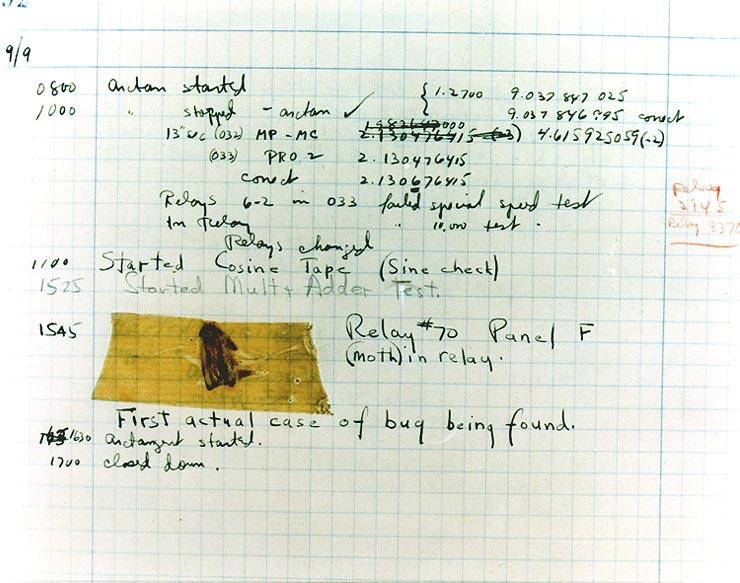
\includegraphics[width=0.62\linewidth]{registro_mark_ii_bug}\\[3pt]
  \begin{minipage}{0.8\linewidth}\centering\footnotesize
    Il registro del calcolatore Harvard Mark II, 9 settembre 1947: alle 15:45 nel relè n.~70 del pannello F si trova una
    falena, attaccata al foglio con la nota «First actual case of bug being found» (immagine delle slide).
  \end{minipage}
\end{center}

È il celebre «bug» di Grace Hopper e del suo gruppo. La nota è una battuta: la parola, nel senso di difetto, era già in
uso (le slide ricordano che il primo impiego si deve probabilmente a Thomas Edison), e quella volta il bug era un
insetto vero.

% ------------------------------------------------------------
\subsection{Defect testing e tesi di Dijkstra}

Il \textbf{defect testing} serve a trovare i difetti di un software, e i difetti si trovano cercando i
malfunzionamenti. Ne segue un paradosso solo apparente: un caso di test \textbf{riesce} quando il programma
\textbf{fallisce}, cioè quando osserviamo un malfunzionamento. Un test che non trova nulla non ha dimostrato che non ci
sono difetti. Il testing, insomma, può dimostrare la \textbf{presenza} dei difetti; può dimostrarne anche
l'\textbf{assenza}?

\dfn{Tesi di Dijkstra}{
  Il testing non può dimostrare l'assenza di difetti, ma solo la loro presenza.}

Non c'è garanzia che, se all'\(n\)-esimo test un modulo o un sistema ha risposto correttamente, lo stesso accada
all'\((n+1)\)-esimo; e non è possibile provare tutte le configurazioni dei valori di input in tutti i possibili stati
interni di un sistema. L'ISTQB (\textit{International Software Testing Qualifications Board}) riassume l'esperienza in
\textbf{sette principi}:

\begin{enumerate}
  \item il testing mostra la presenza dei difetti, non la loro assenza;
  \item il testing esaustivo è (in generale) impossibile;
  \item testare presto fa risparmiare tempo e denaro: prima si scopre un difetto, meno modifiche servono a correggerlo;
  \item i difetti tendono a raggrupparsi, una sorta di principio di località degli accessi;
  \item attenzione al \textbf{paradosso del pesticida}: il codice «si adatta» ai test, e per trovare i nuovi difetti
        introdotti nel tempo servono sempre test nuovi;
  \item il testing dipende dal contesto: non esistono strategie e tecniche universali, valide in ogni situazione;
  \item l'assenza di errori è una falsa credenza, conseguenza pratica dei principi 1 e 2.
\end{enumerate}

Il syllabus dell'ISTQB dà al settimo principio anche un secondo senso: trovare e correggere molti difetti non basta a
garantire il successo di un sistema, se il sistema non soddisfa i bisogni e le aspettative degli utenti. È la
differenza fra verifica e convalida vista sopra.

% ============================================================
\section{Specificare un caso di test}

Un caso di test non è «provare un po' il programma». Per descriverlo serve un insieme minimo di informazioni:

\begin{itemize}
  \item un \textbf{identificativo} (ID) e una descrizione;
  \item le \textbf{precondizioni}: le ipotesi che devono essere vere prima di eseguire il test;
  \item i valori di \textbf{input};
  \item i valori di \textbf{output attesi} (quello che diremo l'«oracolo»);
  \item le \textbf{postcondizioni attese}: le ipotesi che devono essere vere dopo l'esecuzione.
\end{itemize}

Il \textbf{resoconto di esecuzione} aggiunge l'output effettivamente ottenuto e il \textbf{risultato}:

\begin{itemize}
  \item \textbf{successo}, se precondizioni e postcondizioni sono vere e l'output è giudicato equivalente a quello atteso;
  \item \textbf{fallimento}, se precondizioni e postcondizioni sono vere ma l'output \textbf{non} è equivalente a quello
        atteso;
  \item \textbf{non applicabile} (N/A), se almeno una precondizione o una postcondizione non è vera.
\end{itemize}

L'\textbf{input} può avere forme diverse: coppie attributo-valore (i parametri di un metodo, di cui si conoscono nome e
tipo), un flusso di dati (per esempio un file di testo), una sequenza di azioni (in un'applicazione con interfaccia
grafica, la sequenza degli eventi dell'utente, di lunghezza qualsiasi), un insieme di segnali con i loro tempi di arrivo
e di uscita. Per un servizio web si conoscono i nomi delle variabili ma non i tipi dei valori, che viaggiano come
stringhe. Anche l'\textbf{output} può essere un valore o un oggetto (nel test di metodi e servizi) oppure una schermata o
un elemento grafico (nel test di un'interfaccia).

\Needspace{16\baselineskip}
Le slide costruiscono passo passo tre specifiche: un metodo statico, un metodo che cambia lo stato di un oggetto e una
funzione del Blocco note di Windows. Eccole complete:

\begin{center}
\small
\renewcommand{\arraystretch}{1.3}
\begin{tabular}{>{\raggedright\arraybackslash}p{2.6cm}>{\raggedright\arraybackslash}p{3.2cm}%
                >{\raggedright\arraybackslash}p{3.3cm}>{\raggedright\arraybackslash}p{2.3cm}%
                >{\raggedright\arraybackslash}p{2.6cm}}
  \textbf{Unità} & \textbf{Precondizioni} & \textbf{Input} & \textbf{Output atteso} & \textbf{Postcondizioni} \\ \hline
  \texttt{static int sum(int x, int y)} & nessuna & \texttt{x=1}, \texttt{y=2} & \texttt{3} & nessuna \\[2pt]
  \texttt{void increase(}\allowbreak\texttt{Integer x)} della classe \texttt{Count} & esiste un oggetto \texttt{c} di tipo \texttt{Count};
     \texttt{c.value==2} & \texttt{x=new Integer(1)} & nessuno & \texttt{c.value==3} \\[2pt]
  \texttt{notepad.exe}: cercare «pippo» & \texttt{prova.txt} esiste e contiene «pippo» & apri \texttt{prova.txt};
     Modifica; Trova\ldots; digita «pippo»; Trova successivo; esci & il messaggio «pippo found» & il messaggio è
     visibile sullo schermo \\
\end{tabular}
\end{center}

Qualche osservazione:

\begin{itemize}
  \item \texttt{sum} non ha stato: non servono né precondizioni né postcondizioni, e l'output è un \texttt{int};
  \item \texttt{increase} restituisce \texttt{void}: non c'è un output vero e proprio, il metodo cambia lo
        \textbf{stato interno} dell'oggetto, ed è la postcondizione a controllarlo. L'input è un oggetto, specificato
        insieme al costruttore che serve per ottenerlo. (Nella slide sulle precondizioni il metodo è chiamato
        \texttt{triple}: è un residuo di un altro esempio, il metodo è \texttt{increase}.)
  \item nel Blocco note le precondizioni sono due, e devono valere entrambe; la ricerca non modifica il file, quindi le
        postcondizioni non riguardano il file, ma lo \textbf{stato dell'interfaccia}, che serve conoscere per eseguire
        un altro test subito dopo (per esempio una sostituzione di testo). Nei test complessi si aggiungono anche
        condizioni intermedie, per capire meglio \textbf{dove} qualcosa è andato storto.
\end{itemize}

% ------------------------------------------------------------
\subsection{L'oracolo e il comparatore}

L'output effettivo va confrontato con quello atteso per stabilire il risultato del test. Lo fa il
\textbf{comparatore}, che deve valutare in modo \textbf{oggettivo} se i due sono uguali, identici o equivalenti. L'output
atteso lo fornisce l'\textbf{oracolo}, che conosce esattamente come deve rispondere il sistema sotto test a ciascun
caso di test; nel caso più semplice l'oracolo è la colonna degli output attesi di una tabella come quella sopra.

\begin{center}
\begin{tikzpicture}
  \node[tbox=swgray, minimum width=2.3cm, minimum height=0.7cm] (casi) at (2.4,2.2) {Casi di test};
  \node[tbox=swblue, minimum width=2.3cm, minimum height=0.8cm] (sw) at (0,0.9) {Software\\da testare};
  \node[tbox=sworange, minimum width=2.3cm, minimum height=0.8cm] (or) at (4.8,0.9) {Oracolo};
  \node[draw=black!70, fill=swlight, line width=0.7pt, isosceles triangle, isosceles triangle apex angle=60,
        shape border rotate=-90, inner sep=2pt, font=\scriptsize, align=center] (cmp) at (2.4,-0.75)
        {Compa-\\ratore};
  \node[font=\scriptsize\bfseries] (ris) at (2.4,-2.2) {Risultato del test};
  \draw[tfreccia] (casi.south) -- ++(0,-0.35) -| (sw.north);
  \draw[tfreccia] (casi.south) -- ++(0,-0.35) -| (or.north);
  \draw[tfreccia] (sw.south) |- node[tlab, pos=0.25, left] {output} ([yshift=0.25cm]cmp.west);
  \draw[tfreccia] (or.south) |- node[tlab, pos=0.25, right] {output atteso} ([yshift=0.25cm]cmp.east);
  \draw[tfreccia] (cmp.apex) -- (ris.north);
\end{tikzpicture}
\end{center}

Chi può fare da oracolo?

\begin{itemize}
  \item un \textbf{oracolo umano}, che valuta l'esito sulla base dei requisiti e del proprio giudizio, per esempio nel
        test di accettazione;
  \item un \textbf{oracolo software}: un altro programma con lo stesso comportamento di quello sotto test. Una versione
        nota del bubble sort può fare da oracolo per un quicksort più veloce; la versione precedente di un software
        può fare da oracolo per la nuova, che offre le stesse funzionalità (\textbf{test di regressione}). Più avanti
        la libreria \texttt{java.time} farà da oracolo per un programma che calcola il giorno della settimana;
  \item un \textbf{oracolo implicito}: nel test contro i crash, ogni crash è un malfunzionamento;
  \item un \textbf{oracolo da specifica formale}: se i requisiti sono espressi in modo formale, l'oracolo si ricava
        automaticamente da essi.
\end{itemize}

% ============================================================
\section{La qualità dei test}

Una suite di test, come qualunque prodotto, può essere fatta bene o male. I requisiti di qualità dei test sono sette:

\begin{enumerate}
  \item \textbf{accuratezza}: la valutazione del risultato deve essere accurata e oggettiva;
  \item \textbf{ripetibilità}: ripetuti nelle stesse condizioni, i casi di test devono dare ogni volta lo stesso
        risultato;
  \item \textbf{robustezza}: i casi di test dovrebbero restare utilizzabili anche dopo le modifiche al programma;
  \item \textbf{capacità di localizzare i difetti}: un test che fallisce deve guidare il debugging;
  \item \textbf{tracciabilità}: i casi di test devono essere collegati ai requisiti e al progetto;
  \item \textbf{efficacia}: i casi di test dovrebbero trovare tutti i difetti;
  \item \textbf{efficienza}: la suite dovrebbe trovare i difetti con il minor numero di casi di test.
\end{enumerate}

\subsection{Efficacia e copertura}

L'obiettivo principale del testing è trovare il maggior numero di difetti. Una suite \(T_1\) è più efficace di una suite
\(T_2\) se trova più difetti \textbf{diversi}; attenzione però: avere più casi di test che falliscono, o osservare più
malfunzionamenti, non significa trovare più difetti diversi. La strategia ovvia per aumentare l'efficacia è eseguire
sempre più test. L'efficacia si misurerebbe così:
\[
  \text{Efficacia}(T) = \frac{\text{numero di difetti diversi trovati da } T}{\text{numero di difetti esistenti}}
  \qquad
  \text{Efficacia relativa}(T_1, T_2) = \frac{\text{difetti diversi trovati da } T_1}{\text{difetti diversi trovati da }
  T_2}
\]

ma il numero di difetti esistenti in generale non si conosce; il numero di test eseguiti non misura lo sforzo che è
costato eseguirli; e i test che trovano tutti lo stesso difetto non dovrebbero contare. Soprattutto, le misure «esatte»
dipendono dalla presenza reale dei difetti: se un software non ha più bug, efficacia ed efficienza di qualsiasi suite
valgono zero. Non sapendo se ci sono difetti, non si può rinunciare a testare, e servono quindi \textbf{misure
approssimate}, utili anche quando i difetti sono pochi o nessuno. La più usata è la \textbf{copertura del codice}:
\begin{gather*}
  \text{Cov}_{\text{LOC}} = \frac{\text{righe eseguite da almeno un test}}{\text{righe totali}}
  \qquad
  \text{Cov}_{\text{metodi}} = \frac{\text{metodi chiamati da almeno un test}}{\text{metodi totali}}
  \\[4pt]
  \text{Cov}_{\text{classi}} = \frac{\text{classi usate da almeno un test}}{\text{classi totali}}
\end{gather*}

Il ragionamento è semplice: se una riga contiene un difetto e nessun test la esegue, il difetto \textbf{di sicuro} non
verrà trovato; se qualche test la esegue, è \textbf{possibile} che il difetto causi un malfunzionamento. In generale più
codice si esegue, più cresce la «speranza» di trovare difetti; e se due suite trovano lo stesso numero di difetti
(magari zero) e \(T_1\) copre più righe di \(T_2\), si può avere più fiducia in \(T_1\). Con il carrello della
sezione su JUnit si vedrà però che il 100\% delle righe non basta: un ramo può restare scoperto.

% ============================================================
\section{Classificare il testing}

Le classificazioni possibili sono molte: rispetto alla tecnica, all'oggetto sotto test, alle proprietà provate, al
processo. Anche gli standard ne propongono di diverse. Lo standard IEEE 29119 usa quattro dimensioni: le
\textbf{tecniche} di verifica e convalida, i \textbf{livelli} di test, i \textbf{processi} (o pratiche) e le
\textbf{proprietà} provate (i tipi di test).

\Needspace{30\baselineskip}
\begin{center}
\small
\renewcommand{\arraystretch}{1.15}
\begin{tabular}{>{\raggedright\arraybackslash}p{2.5cm}>{\raggedright\arraybackslash}p{3.3cm}%
                >{\raggedright\arraybackslash}p{9.2cm}}
  \multicolumn{3}{l}{\textbf{Tecniche di verifica e convalida}} \\ \hline
  Test statico & & revisioni (\textit{review}), verifica dei modelli, analisi statica \\ \hline
  Test dinamico & basato sulla specifica & partizione in classi di equivalenza, \textit{classification tree method},
    analisi dei valori limite, \textit{syntax testing}, progettazione combinatoria (tutte le combinazioni,
    \textit{pair-wise}, \textit{each choice}, \textit{base choice}), tabelle di decisione, grafi causa-effetto,
    test delle transizioni di stato, test di scenario, test casuale \\
  & basato sulla struttura & test delle istruzioni, dei rami, delle decisioni, delle condizioni dei rami e delle
    loro combinazioni, MC/DC (\textit{Modified Condition Decision Coverage}), test del flusso dei dati (\textit{all
    definitions}, \textit{all c-uses}, \textit{all p-uses}, \textit{all uses}, \textit{all DU-paths}) \\
  & basato sull'esperienza & \textit{error guessing} \\ \hline
  Dimostrazione & & prototipi, prove con gli utenti, mock-up \\ \hline
  Analisi & & metodi formali (\textit{model checking}, dimostrazione di correttezza), simulazione, valutazione con
    metriche di qualità \\
\end{tabular}
\end{center}

I \textbf{livelli} di test sono: test di \textbf{unità}, di \textbf{integrazione}, di \textbf{sistema}, di integrazione
di sistemi e di \textbf{accettazione} (dell'utente, operativa, in fabbrica, \textit{alpha}, \textit{beta}, di verifica
in produzione).

\begin{itemize}
  \item L'\textbf{unità} è per definizione la parte più piccola del software che si intende testare, e coincide con il
        concetto di modulo usato nel progetto: una funzione, un metodo, una classe, un package (attraverso la sua
        interfaccia), al limite l'intero sistema. Il test di unità si può condurre a \textbf{scatola nera}, se si
        conosce solo la specifica dell'unità (input, output, funzione realizzata), o a \textbf{scatola bianca}, se si
        conosce anche come è fatta e si vuole sfruttare questa conoscenza.
  \item Un'unità si può testare solo se la si può \textbf{isolare} dal resto del sistema: l'isolamento si ottiene
        sostituendo i componenti o i servizi da cui dipende con dei \textbf{test double} (\textit{mock} o
        \textit{stub}). Il test di \textbf{integrazione} prova il sistema pezzo per pezzo, eventualmente con l'aiuto
        dei test double.
  \item Il test di \textbf{sistema} prova il software nella sua interezza, per esempio interagendo con l'interfaccia
        utente e osservando i risultati sull'interfaccia e, per esempio, nei database o nei file.
\end{itemize}

Fra le \textbf{pratiche} lo standard elenca il test basato sui modelli, il test con script, il test esplorativo e
quello basato sull'esperienza, il test manuale, l'A/B testing, il \textit{back-to-back testing}, il test su base
matematica, il \textit{fuzz testing}, il \textit{keyword-driven testing} e il test automatico (\textit{capture-replay} e
\textit{data-driven}). Fra i \textbf{tipi} di test (le proprietà provate): funzionale, di accessibilità, di
compatibilità, di \textit{disaster recovery}, di installabilità, di interoperabilità, di localizzazione, di
manutenibilità, di prestazioni (prestazioni, carico, stress, capacità, ripristino), di portabilità, di procedura, di
affidabilità, di sicurezza e di usabilità.

% ============================================================
\section{Testing a scatola nera}

Il \textbf{principio di verificabilità dei requisiti} chiede che i requisiti siano testabili: scritti in modo che si
possano progettare test capaci di dimostrare che il requisito è soddisfatto. Il \textbf{test basato sui requisiti} è una
tecnica di convalida che progetta diversi test per ogni requisito. In generale il test basato sulla specifica rientra
nella grande famiglia del \textbf{testing a scatola nera} (\textit{black box}): i casi di test si progettano
\textbf{senza alcuna informazione interna} sul sistema sotto test, solo a partire dalla sua specifica.

Un esempio è il \textbf{test degli scenari dei casi d'uso}: dato il diagramma dei casi d'uso (Capitolo~6) con la
descrizione di tutti gli scenari, per ogni scenario si progettano uno o più casi di test che lo eseguono, da lanciare a
mano o in modo automatico; l'obiettivo è coprire i casi d'uso e i loro scenari.

Gli approcci sono due, complementari:

\begin{itemize}
  \item nel test \textbf{basato sui requisiti} i casi di test nascono dall'analisi dei comportamenti da verificare; la
        difficoltà è trovare i valori di test capaci di provocarli;
  \item nelle tecniche di \textbf{partizione del dominio di input} (il \textit{data-driven testing}) i casi di test
        nascono per coprire combinazioni di valori di input; la difficoltà è coprire i comportamenti
        dell'applicazione con il minor numero possibile di casi di test.
\end{itemize}

% ------------------------------------------------------------
\subsection{Partizione in classi di equivalenza}

I valori di un campo di input si possono dividere in classi i cui elementi sono in qualche modo legati fra loro: ogni
classe è una \textbf{classe di equivalenza}. L'ipotesi è che il programma si comporti \textbf{allo stesso modo} per tutti
gli elementi di una classe; i casi di test sono allora una selezione di valori presi dalle classi, e i criteri di
copertura si definiscono sulla copertura delle classi di ciascun input.

\dfn{Classi di equivalenza}{
  Le classi di equivalenza di un input formano una \textbf{partizione} del suo dominio: la loro unione è l'intero
  dominio di input, e due classi non hanno elementi in comune.}

\Needspace{14\baselineskip}
\begin{center}
\begin{tikzpicture}
  \node[draw=swblue!70!black, fill=swblue!6, ellipse, minimum width=6.6cm, minimum height=1.9cm, line width=0.7pt]
    (in) at (0,0) {};
  \node[font=\scriptsize\bfseries, text=swblue!80!black] at (0,-0.65) {dominio di input};
  \foreach \x/\c in {-2.2/swred, -1.6/swred, 0.4/swgreen, 1.1/swgreen, 1.8/swgreen}{
    \node[draw=\c!75!black, fill=\c!15, ellipse, minimum width=0.62cm, minimum height=0.42cm, line width=0.6pt]
      at (\x,0.2) {};}
  \node[font=\tiny, text=swred!80!black] at (-1.9,0.62) {classi non valide};
  \node[font=\tiny, text=swgreen!70!black] at (1.1,0.62) {classi valide};
  \node[tbox=swgray, minimum width=2.4cm] (sys) at (0,-1.9) {Sistema};
  \node[draw=sworange!80!black, fill=sworange!8, ellipse, minimum width=4.2cm, minimum height=1.1cm,
        line width=0.7pt, font=\scriptsize] (out) at (0,-3.4) {output};
  \draw[tfreccia] (in.south) -- (sys.north);
  \draw[tfreccia] (sys.south) -- (out.north);
\end{tikzpicture}
\end{center}

\Needspace{12\baselineskip}
\subsubsection*{L'esempio del calendario}

Un metodo riceve una data, composta da giorno (intero), mese (stringa) e anno (intero). Deve distinguere le date
valide (giorni che sono esistiti davvero) da quelle non valide, e restituisce un booleano (vero se la data è valida) e
una stringa: il giorno della settimana, oppure «Errore» se la data non è valida. Le informazioni sul dominio vengono dal
calendario gregoriano:

\begin{itemize}
  \item i mesi hanno durate diverse;
  \item il 29 febbraio esiste solo negli anni bisestili;
  \item sono bisestili gli anni divisibili per 4 ma non per 100 \textbf{salvo quelli divisibili per 400}: il 2000 è
        bisestile, il 1900 no (le slide si fermano a «divisibili per 4 ma non per 100», ma il codice che vedremo
        applica la regola completa);
  \item il calendario è entrato in vigore il 15 ottobre 1582 (al 4 ottobre seguì direttamente il 15).
\end{itemize}

Gli input sono quindi il \textbf{giorno}, un intero in un intervallo limitato in basso e in alto; il \textbf{mese}, una
stringa in un insieme di 12 valori; l'\textbf{anno}, un intero limitato solo in basso. Gli output sono la
\textbf{validità}, un booleano, e il \textbf{giorno della settimana}, una stringa con 7 valori validi più quello di
errore. Le slide introducono i vincoli a poco a poco, per ragioni didattiche.

Le classi di equivalenza si possono definire con due approcci:

\begin{enumerate}
  \item \textbf{basato sull'interfaccia}: ogni parametro è considerato da solo, e per ciascuno si progettano le sue
        classi;
  \item \textbf{basato sulla funzionalità}: si individuano le caratteristiche che corrispondono alla funzionalità
        attesa; le classi riflettono il comportamento atteso e tengono conto delle relazioni fra i parametri. Il
        modello si basa sui \textbf{requisiti}, non sull'implementazione.
\end{enumerate}

\subsubsection*{L'approccio basato sull'interfaccia}

Le partizioni si ricavano dalla specifica o da altra documentazione; ogni classe rappresenta un insieme di valori di un
input, nell'ipotesi che il sistema si comporti allo stesso modo per tutti i valori della stessa classe. Per ogni input
si ottengono \textbf{una o più classi valide} (i valori accettabili) e \textbf{un insieme di classi non valide}, una per
ogni condizione di non validità. Si considera un input alla volta, ignorando le interazioni fra gli input. I casi tipici:

\begin{itemize}
  \item \textbf{intervallo di valori}: una classe valida per i valori nell'intervallo, una non valida per quelli sotto
        il minimo e una per quelli sopra il massimo;
  \item \textbf{valore specifico}: una classe valida per quel valore, una non valida per i valori minori e una per
        quelli maggiori;
  \item \textbf{elemento di un insieme discreto}: una classe valida per l'intero insieme (test minimo) o una per ogni
        elemento (test dettagliato), più una non valida per gli elementi fuori dall'insieme;
  \item \textbf{valore booleano}: come il caso precedente, con un insieme di due valori.
\end{itemize}

In alcuni casi conviene una classe non valida in più, con tutti i valori rimanenti che si potrebbero passare. Per il
calendario, con il minimo delle informazioni:

\begin{itemize}
  \item \textbf{giorno}, intero fra 1 e 31: \(\{giorno \le 0\}\), \(\{1 \le giorno \le 31\}\), \(\{giorno > 31\}\);
  \item \textbf{mese}, una stringa fra 12: \(\{mese \in \{\text{gennaio}, \ldots, \text{dicembre}\}\}\),
        \(\{mese \notin \{\text{gennaio}, \ldots, \text{dicembre}\}\}\);
  \item \textbf{anno}, intero da 1582 in su: \(\{anno < 1582\}\), \(\{anno \ge 1582\}\).
\end{itemize}

Ci sono poi le classi dei valori \textbf{di tipo sbagliato}, per esempio una stringa come giorno. Servono quando il
sistema non controlla i tipi (un flusso di input, un form web, un protocollo), ma non nel test di unità di un linguaggio
compilato: il compilatore impedirebbe di chiamare il metodo con un argomento del tipo sbagliato.

\warning{Classi e casi di test}{
  Le classi di equivalenza sono \textbf{insiemi} di possibili valori di test; un caso di test specifica \textbf{un
  valore} per ogni input. La classe a cui appartiene il valore scelto risulta coperta dal caso di test.}

\subsubsection*{Criteri di copertura delle classi}

Fissate le classi, si possono definire criteri di test che mirano a coprirle in modi diversi:

\begin{itemize}
  \item \textbf{Each Choice Coverage} (ECC), la copertura minima: ogni classe è coperta da almeno un caso di test. Il
        numero minimo di casi di test è pari al massimo numero di classi di un singolo input (qui 3, per il giorno);
  \item \textbf{All Combinations Coverage} (ACC): si coprono tutte le combinazioni delle classi; il numero di casi di
        test è il prodotto del numero di classi di ciascun input (qui \(3 \cdot 2 \cdot 2 = 12\)). Corrisponde al caso
        \(t\)-\textit{wise} con \(t\) pari al numero degli input.
\end{itemize}

\Needspace{12\baselineskip}
Ecco i casi delle slide per ECC (con i mesi in inglese, come nell'esempio dell'interfaccia):

\begin{center}
\renewcommand{\arraystretch}{1.2}
\begin{tabular}{lcccc}
  \textbf{Caso di test} & \textbf{TC1} & \textbf{TC2} & \textbf{TC3} & \textbf{TC4} \\ \hline
  Giorno & 1 & 0 & 35 & first \\
  Mese & January & Brumaire & January & January \\
  Anno & 1980 & 1492 & 1980 & two thousand \\
\end{tabular}
\end{center}

TC4 copre le classi di tipo sbagliato e in Java si omette. Per eseguire davvero questi casi serve un'implementazione: si
usa quella che le slide presentano più avanti, nella parte sull'integrazione, che vuole i mesi in italiano (Brumaire,
il mese «delle brume» del calendario rivoluzionario francese, diventa «brumaio»). Qui il metodo
\texttt{giornoDellaSettimana(giorno, mese, anno)} è trattato davvero come una scatola nera: il suo codice si vedrà solo
più avanti. I casi diventano un test \textbf{parametrico} di JUnit~4 (il funzionamento di JUnit è spiegato nella sezione
che gli è dedicata): il metodo \texttt{casi()} elenca le righe della tabella, con l'output atteso scritto a mano, e
JUnit esegue il test una volta per riga.

\Needspace{40\baselineskip}
\begin{lstlisting}[style=java, name=CalendarioECCTest.java]
import static org.junit.Assert.assertEquals;

import java.util.Arrays;
import java.util.Collection;

import org.junit.Test;
import org.junit.runner.RunWith;
import org.junit.runners.Parameterized;
import org.junit.runners.Parameterized.Parameters;

// Each Choice Coverage: ogni classe di equivalenza in almeno un caso di test
@RunWith(Parameterized.class)
public class CalendarioECCTest {

    @Parameters(name = "{0} {1} {2,number,#} -> {3}")
    public static Collection<Object[]> casi() {
        return Arrays.asList(new Object[][] {
            {1, "gennaio", 1980, "Martedi"},   // TC1: giorno, mese e anno validi
            {0, "brumaio", 1492, "Errore"},    // TC2: tutti e tre non validi
            {35, "gennaio", 1980, "Errore"},   // TC3: giorno oltre il massimo
        });
    }

    private final int giorno;
    private final String mese;
    private final int anno;
    private final String atteso;

    public CalendarioECCTest(int giorno, String mese, int anno, String atteso) {
        this.giorno = giorno;
        this.mese = mese;
        this.anno = anno;
        this.atteso = atteso;
    }

    @Test
    public void testGiornoDellaSettimana() {
        assertEquals(atteso, Calendario.giornoDellaSettimana(giorno, mese, anno));
    }
}
\end{lstlisting}

\Needspace{16\baselineskip}
Il test per ACC è identico, tranne il metodo \texttt{casi()}, che genera le 12 combinazioni con tre cicli annidati. Si
noti che anche l'oracolo va scritto: qui è una regola fatta a mano (la data è valida solo se tutte e tre le classi lo
sono), e il 1° gennaio 1980 era un martedì.

\begin{lstlisting}[style=java, name=CalendarioACCTest.java, firstnumber=15]
    @Parameters(name = "{0} {1} {2,number,#} -> {3}")
    public static Collection<Object[]> casi() {
        Collection<Object[]> casi = new ArrayList<>();
        for (int anno : new int[] {1980, 1492})
            for (String mese : new String[] {"gennaio", "brumaio"})
                for (int giorno : new int[] {1, 0, 35}) {
                    // l'oracolo, scritto a mano: valida solo la combinazione di classi valide
                    boolean valida = giorno == 1 && mese.equals("gennaio") && anno == 1980;
                    casi.add(new Object[] {giorno, mese, anno, valida ? "Martedi" : "Errore"});
                }
        return casi;
    }
\end{lstlisting}

\Needspace{20\baselineskip}
Con Maven si sceglie quali classi di test eseguire con \texttt{-Dtest}:

\begin{lstlisting}[style=shell, name=Terminale]
$ mvn test -Dtest='CalendarioECCTest,CalendarioACCTest'
...
[INFO] -------------------------------------------------------
[INFO]  T E S T S
[INFO] -------------------------------------------------------
[INFO] Running CalendarioACCTest
[INFO] Tests run: 12, Failures: 0, Errors: 0, Skipped: 0, Time elapsed: 0.060 s -- in CalendarioACCTest
[INFO] Running CalendarioECCTest
[INFO] Tests run: 3, Failures: 0, Errors: 0, Skipped: 0, Time elapsed: 0.005 s -- in CalendarioECCTest
[INFO]
[INFO] Results:
[INFO]
[INFO] Tests run: 15, Failures: 0, Errors: 0, Skipped: 0
...
[INFO] ------------------------------------------------------------------------
[INFO] BUILD SUCCESS
\end{lstlisting}

I 15 casi passano: per queste classi il metodo si comporta come previsto.

\subsubsection*{L'approccio basato sulla funzionalità}

Ora si sfrutta di più la conoscenza del comportamento atteso, non solo dell'interfaccia. Per esempio: ci sono mesi che
possono avere solo 28, 29, 30 o 31 giorni. Le classi di giorno e mese diventano più fini:

\begin{itemize}
  \item \textbf{giorno}: \(\{giorno \le 0\}\), \(\{1 \le giorno \le 28\}\), \(\{giorno = 29\}\), \(\{giorno = 30\}\),
        \(\{giorno = 31\}\), \(\{giorno > 31\}\): 6 classi;
  \item \textbf{mese}: i mesi di 31 giorni (gennaio, marzo, maggio, luglio, agosto, ottobre, dicembre), quelli di 30
        (aprile, giugno, settembre, novembre), febbraio, e le stringhe che non sono mesi: 4 classi;
  \item \textbf{anno}: \(\{anno < 1582\}\), \(\{anno = 1582\}\), \(\{anno > 1582\}\): 3 classi.
\end{itemize}

Con ACC servirebbero ora \(6 \cdot 4 \cdot 3 = 72\) casi di test.

% ------------------------------------------------------------
\subsection{Analisi dei valori limite}

Una variante della tecnica delle classi di equivalenza considera i \textbf{valori limite} (\textit{boundary values}):
classi aggiuntive, valide e non valide, che corrispondono agli estremi degli insiemi di validità. Di solito riguardano
gli intervalli, ma sono valori limite anche quelli per cui si sospetta un comportamento particolare in qualche
operazione, come lo zero per un intero che potrebbe finire a denominatore, o per un puntatore. Se la condizione su un
input specifica:

\begin{itemize}
  \item un \textbf{intervallo chiuso}: sono classi limite il minimo e il massimo (valide) e i valori appena sotto il
        minimo e appena sopra il massimo (non valide); con più intervalli il ragionamento si ripete per ciascuno;
  \item un \textbf{intero}: una classe limite, qualunque sia la specifica, è \(\{0\}\); un'altra, salvo indicazioni
        diverse, è quella dei numeri negativi.
\end{itemize}

Per il calendario, le slide elencano dodici classi limite per il giorno: \(\{giorno \ll 0\}\), \(\{0\}\) (appena sotto
il minimo, e anche valore nullo), \(\{1\}\) (il minimo), \(\{2\}\), un valore lontano dagli estremi, \(\{27\}\),
\(\{28\}\) (il massimo in certi casi), \(\{29\}\), \(\{30\}\) e \(\{31\}\) (valori critici ben noti), \(\{32\}\) e
\(\{giorno \gg 31\}\). Per l'anno: \(\{anno \ll 1582\}\), \(\{1581\}\), \(\{1582\}\) (estremo inferiore e valore
critico), \(\{1583\}\) e un valore molto più grande. Per il mese, una classe per ciascuno dei dodici mesi più quella
delle stringhe che non sono mesi. (Nelle slide la prima classe dell'anno è scritta \(\{Day \ll 1582\}\), con
\textit{Day} al posto di \textit{Year}, e l'ultima è descritta come «sopra l'estremo superiore», che per l'anno non
esiste: è semplicemente un valore lontano dall'estremo inferiore.)

\Needspace{30\baselineskip}
Un test parametrico con una selezione di questi valori, gli output attesi ricavati dal calendario:

\begin{lstlisting}[style=java, name=CalendarioLimitiTest.java, firstnumber=15]
    @Parameters(name = "{0} {1} {2,number,#} -> {3}")
    public static Collection<Object[]> casi() {
        return Arrays.asList(new Object[][] {
            {0, "gennaio", 2011, "Errore"},       // appena sotto il minimo
            {1, "gennaio", 2011, "Sabato"},       // minimo
            {31, "gennaio", 2011, "Lunedi"},      // massimo di un mese di 31 giorni
            {32, "gennaio", 2011, "Errore"},      // appena sopra il massimo
            {30, "aprile", 2011, "Sabato"},       // massimo di un mese di 30 giorni
            {31, "aprile", 2011, "Errore"},
            {28, "febbraio", 2011, "Lunedi"},     // febbraio, anno non bisestile
            {29, "febbraio", 2011, "Errore"},
            {29, "febbraio", 2012, "Mercoledi"},  // anno bisestile
            {29, "febbraio", 1900, "Errore"},     // divisibile per 100: non bisestile
            {29, "febbraio", 2000, "Martedi"},    // divisibile per 400: bisestile
            {14, "ottobre", 1582, "Errore"},      // giorno saltato dalla riforma
            {15, "ottobre", 1582, "Venerdi"},     // primo giorno del calendario gregoriano
            {1, "gennaio", 1583, "Sabato"},
        });
    }
\end{lstlisting}

\begin{lstlisting}[style=shell, name=Terminale, deletekeywords={java}]
$ mvn test -Dtest=CalendarioLimitiTest
...
[INFO] -------------------------------------------------------
[INFO]  T E S T S
[INFO] -------------------------------------------------------
[INFO] Running CalendarioLimitiTest
[ERROR] Tests run: 14, Failures: 1, Errors: 0, Skipped: 0, Time elapsed: 0.075 s <<< FAILURE! -- in CalendarioLimitiTest
[ERROR] CalendarioLimitiTest.testGiornoDellaSettimana[15 ottobre 1582 -> Venerdi] -- Time elapsed: 0.007 s <<< FAILURE!
org.junit.ComparisonFailure: expected:<[Venerdi]> but was:<[Errore]>
    at org.junit.Assert.assertEquals(Assert.java:117)
    at org.junit.Assert.assertEquals(Assert.java:146)
    at CalendarioLimitiTest.testGiornoDellaSettimana(CalendarioLimitiTest.java:49)
    at java.base/java.lang.reflect.Method.invoke(Method.java:580)

[INFO]
[INFO] Results:
[INFO]
[ERROR] Failures:
[ERROR]   CalendarioLimitiTest.testGiornoDellaSettimana:49 expected:<[Venerdi]> but was:<[Errore]>
[INFO]
[ERROR] Tests run: 14, Failures: 1, Errors: 0, Skipped: 0
[INFO]
[INFO] ------------------------------------------------------------------------
[INFO] BUILD FAILURE
\end{lstlisting}

I valori limite hanno trovato un difetto che le classi di equivalenza dell'interfaccia non vedevano: il 15 ottobre
1582, primo giorno del calendario gregoriano (un venerdì), viene rifiutato come data non valida. Il motivo, quando si
leggerà il codice, sarà la condizione \texttt{a <= 1582}, che esclude l'intero 1582. I casi su febbraio, invece,
confermano che la regola dei bisestili è applicata per intero (il 29 febbraio 2000 esiste, il 29 febbraio 1900 no).

\subsubsection*{Un oracolo software}

Quante date sono sbagliate, esattamente? Con un \textbf{oracolo software} si può controllare ogni data di un lungo
periodo: la libreria \texttt{java.time} di Java sa che giorno della settimana era una data qualsiasi. Il programma che
segue (non è nelle slide) confronta il metodo con l'oracolo per tutti i giorni da 0 a 32 di tutti i mesi dal 1580 al
2100, e stampa le prime discrepanze:

\Needspace{38\baselineskip}
\begin{lstlisting}[style=java, name=Oracolo.java]
import java.time.DateTimeException;
import java.time.DayOfWeek;
import java.time.LocalDate;

public class Oracolo {
    static final String[] MESI = {"gennaio", "febbraio", "marzo", "aprile", "maggio", "giugno", "luglio",
            "agosto", "settembre", "ottobre", "novembre", "dicembre"};
    static final String[] GIORNI = {"Lunedi", "Martedi", "Mercoledi", "Giovedi", "Venerdi", "Sabato", "Domenica"};

    public static void main(String[] args) {
        int date = 0, giorniSbagliati = 0, validitaSbagliate = 0;
        for (int a = 1580; a <= 2100; a++)
            for (int m = 1; m <= 12; m++)
                for (int d = 0; d <= 32; d++) {
                    String atteso;
                    try {
                        LocalDate data = LocalDate.of(a, m, d);
                        atteso = data.isBefore(LocalDate.of(1582, 10, 15)) ? "Errore"
                                : GIORNI[data.getDayOfWeek().getValue() - 1];
                    } catch (DateTimeException e) {
                        atteso = "Errore";
                    }
                    String ottenuto = Calendario.giornoDellaSettimana(d, MESI[m - 1], a);
                    date++;
                    if (!atteso.equals(ottenuto)) {
                        if (atteso.equals("Errore") || ottenuto.equals("Errore")) validitaSbagliate++;
                        else giorniSbagliati++;
                        if (validitaSbagliate + giorniSbagliati <= 3)
                            System.out.println(d + " " + MESI[m - 1] + " " + a + ": atteso " + atteso + ", ottenuto " + ottenuto);
                    }
                }
        System.out.println("date provate: " + date + ", giorno sbagliato: " + giorniSbagliati
                + ", validita' sbagliata: " + validitaSbagliate);
    }
}
\end{lstlisting}

\begin{lstlisting}[style=shell, name=Terminale, deletekeywords={java}, deletestring={[b]'}]
$ javac Oracolo.java
$ java Oracolo
15 ottobre 1582: atteso Venerdi, ottenuto Errore
16 ottobre 1582: atteso Sabato, ottenuto Errore
17 ottobre 1582: atteso Domenica, ottenuto Errore
date provate: 206316, giorno sbagliato: 0, validita' sbagliata: 78
\end{lstlisting}

Su 206\,316 date provate il giorno della settimana non è mai sbagliato; le 78 discrepanze sono proprio i giorni dal 15
ottobre al 31 dicembre 1582 (17 + 30 + 31), tutti rifiutati. (\texttt{LocalDate} usa il calendario gregoriano anche
prima della riforma, per questo le date precedenti al 15 ottobre 1582 sono escluse a mano.)

\subsection{Il problema dell'oracolo}

La generazione automatica di casi di test combinatori non comprende la definizione degli oracoli: vanno aggiunti a mano,
e il costo del testing cresce fino a diventare insostenibile. Nell'esempio di ACC l'oracolo era una regola banale, e qui
sopra c'era a disposizione una libreria affidabile; ma di solito non va così. La tecnica resta praticabile in problemi
specifici:

\begin{itemize}
  \item il \textbf{crash testing}: l'oracolo, valutato in modo del tutto automatico, è la terminazione regolare del
        programma (ci sarebbe anche da considerare il caso in cui non termina\ldots);
  \item la violazione di \textbf{invarianti}: violazioni di sicurezza o di privacy, uso eccessivo di memoria, violazioni
        delle regole di usabilità, e così via.
\end{itemize}

% ============================================================
\section{Testing a scatola bianca}

Il testing a \textbf{scatola bianca} (\textit{white box}) è un test \textbf{strutturale}: usa la conoscenza della
struttura interna del programma per ricavare i dati di test. Osservare l'esecuzione a livello di codice fornisce anche
criteri \textbf{oggettivi} per valutare l'efficacia dei casi di test (le metriche di copertura) e informazioni molto
utili per localizzare i difetti.

La differenza con la scatola nera sta nell'obiettivo. Il testing funzionale (\textit{black box}) cerca di coprire il
maggior numero possibile di \textbf{comportamenti} dell'applicazione, in base a ciò che si sa dei modi in cui si può
interagire con essa (per esempio variando i valori di input). Il testing strutturale (\textit{white box}) cerca invece di
\textbf{eseguire} la maggior parte possibile del codice, per poterlo provare tutto.

\subsection{Il grafo del flusso di controllo}

Molte parti di un sistema software si modellano con dei grafi: gli algoritmi (diagrammi di flusso), i metodi e le
funzioni (grafi del flusso di controllo), le interazioni fra classi (diagrammi degli oggetti), i diagrammi delle
attività, le macchine a stati finiti, i diagrammi degli stati. Per il codice sorgente si usa il \textbf{grafo del
flusso di controllo} (\textit{Control-Flow Graph}, CFG).

\dfn{Grafo del flusso di controllo}{
  Il CFG di un programma (metodo o funzione) \(P\) è la quadrupla \(\mathrm{CFG}(P) = \langle N, A_C, n_I, n_F
  \rangle\), dove:
  \begin{itemize}
    \item \(\langle N, A_C\rangle\) è un grafo orientato con archi etichettati, con \(\{n_I, n_F\} \subseteq N\) e
          \(N \setminus \{n_I, n_F\} = N_s \cup N_p\), dove \(N_s\) (nodi \textbf{istruzione}) e \(N_p\) (nodi
          \textbf{predicato}, cioè le decisioni) sono insiemi disgiunti;
    \item \(A_C \subseteq (N \setminus \{n_F\}) \times (N \setminus \{n_I\}) \times \{\mathit{true}, \mathit{false},
          \mathit{incond}\}\) è la relazione di flusso di controllo;
    \item \(n_I\) e \(n_F\) sono il nodo iniziale e il nodo finale.
  \end{itemize}
  Un nodo di \(N_s \cup \{n_I\}\) ha un solo successore, con l'arco etichettato \(\mathit{incond}\) (incondizionato);
  un nodo di \(N_p\) ha due successori, con gli archi etichettati \(\mathit{true}\) e \(\mathit{false}\).}

\Needspace{22\baselineskip}
Ecco come si traducono le strutture di controllo. I numeri dei nodi sono quelli delle righe del codice; il pallino
pieno è il nodo iniziale, quello cerchiato il nodo finale, e i nodi predicato sono in arancione.

\begin{center}
\begin{tikzpicture}[node distance=0.82cm]
  % --- if ---
  \node[font=\scriptsize\FiraCodeNL, align=left, anchor=north west] at (-1.2,0.3)
    {1. if (decisione)\\2. \{\\3. \ \ Blocco\\4. \}};
  \begin{scope}[shift={(0.3,-1.6)}]
    \node[iniziale] (i) at (0,0) {};
    \node[tdec, below=0.45cm of i] (n1) {1};
    \node[tnodo, below of=n1] (n2) {2};
    \node[tnodo, below of=n2] (n3) {3};
    \node[tnodo, below of=n3] (n4) {4};
    \node[finale, below=0.45cm of n4] (f) {};
    \draw[tarco] (i) -- (n1);
    \draw[tarco] (n1) -- node[tlab, left] {vero} (n2);
    \draw[tarco] (n2) -- (n3); \draw[tarco] (n3) -- (n4); \draw[tarco] (n4) -- (f);
    \draw[tarco] (n1.east) -- ++(0.55,0) |- node[tlab, pos=0.25, right] {falso} (f.east);
  \end{scope}
  % --- if-else ---
  \node[font=\scriptsize\FiraCodeNL, align=left, anchor=north west] at (2.4,0.3)
    {1. if (decisione)\\2. \{\\3. \ \ Blocco1\\4. \}\\5. else\\6. \{\\7. \ \ Blocco2\\8. \}};
  \begin{scope}[shift={(4.6,-1.6)}]
    \node[iniziale] (i) at (0,0) {};
    \node[tdec, below=0.45cm of i] (m1) {1};
    \node[tnodo, below left=0.55cm and 0.35cm of m1] (m2) {2};
    \node[tnodo, below of=m2] (m3) {3};
    \node[tnodo, below of=m3] (m4) {4};
    \node[tnodo, below right=0.55cm and 0.35cm of m1] (m6) {6};
    \node[tnodo, below of=m6] (m7) {7};
    \node[tnodo, below of=m7] (m8) {8};
    \node[finale] (f) at ($(m4)!0.5!(m8)+(0,-0.9)$) {};
    \draw[tarco] (i) -- (m1);
    \draw[tarco] (m1) -- node[tlab, above left] {vero} (m2);
    \draw[tarco] (m1) -- node[tlab, above right] {falso} (m6);
    \draw[tarco] (m2) -- (m3); \draw[tarco] (m3) -- (m4);
    \draw[tarco] (m6) -- (m7); \draw[tarco] (m7) -- (m8);
    \draw[tarco] (m4) -- (f); \draw[tarco] (m8) -- (f);
  \end{scope}
  % --- while ---
  \node[font=\scriptsize\FiraCodeNL, align=left, anchor=north west] at (7.0,0.3)
    {1. while (decisione)\\2. \{\\3. \ \ Blocco\\4. \}};
  \begin{scope}[shift={(8.4,-1.6)}]
    \node[iniziale] (i) at (0,0) {};
    \node[tdec, below=0.45cm of i] (w1) {1};
    \node[tnodo, below of=w1] (w2) {2};
    \node[tnodo, below of=w2] (w3) {3};
    \node[tnodo, below of=w3] (w4) {4};
    \node[finale, below=0.45cm of w4] (f) {};
    \draw[tarco] (i) -- (w1);
    \draw[tarco] (w1) -- node[tlab, right] {vero} (w2);
    \draw[tarco] (w2) -- (w3); \draw[tarco] (w3) -- (w4);
    \draw[tarco] (w4.west) -- ++(-0.45,0) |- (w1.west);
    \draw[tarco] (w1.east) -- ++(0.5,0) |- node[tlab, pos=0.25, right] {falso} (f.east);
  \end{scope}
  % --- do-while ---
  \node[font=\scriptsize\FiraCodeNL, align=left, anchor=north west] at (10.5,0.3)
    {1. do\\2. \{\\3. \ \ Blocco\\4. \}\\5. while (decisione)};
  \begin{scope}[shift={(12.4,-1.6)}]
    \node[iniziale] (i) at (0,0) {};
    \node[tnodo, below=0.45cm of i] (d1) {1};
    \node[tnodo, below of=d1] (d2) {2};
    \node[tnodo, below of=d2] (d3) {3};
    \node[tnodo, below of=d3] (d4) {4};
    \node[tdec, below of=d4] (d5) {5};
    \node[finale, below=0.45cm of d5] (f) {};
    \draw[tarco] (i) -- (d1);
    \draw[tarco] (d1) -- (d2); \draw[tarco] (d2) -- (d3); \draw[tarco] (d3) -- (d4); \draw[tarco] (d4) -- (d5);
    \draw[tarco] (d5.west) -- ++(-0.45,0) |- node[tlab, pos=0.25, left] {vero} (d1.west);
    \draw[tarco] (d5) -- node[tlab, right] {falso} (f);
  \end{scope}
\end{tikzpicture}
\end{center}

Un CFG si può costruire da due punti di vista: a livello di \textbf{codice sorgente} o a livello di \textbf{eseguibile}
(o di bytecode). Pensando all'eseguibile, i nodi 2, 4, 6 e 8 (le parentesi graffe) si possono omettere, perché non
corrispondono ad alcuna istruzione. A livello di sorgente è più facile progettare test che eseguano parti precise del
codice, e il grafo è più compatto e leggibile; a livello di eseguibile il grafo rappresenta esattamente ciò che viene
eseguito.

\Needspace{16\baselineskip}
Il ciclo \texttt{for} mostra bene la differenza. A livello di sorgente la riga 1 è un'unica decisione, come in un
\texttt{while}; a livello di eseguibile ogni \texttt{for} corrisponde a un'inizializzazione \texttt{init} eseguita una
volta, a una decisione \texttt{cond} all'inizio di ogni giro e a un codice di continuazione \texttt{cont} (per esempio
\texttt{i++}) da eseguire prima di ricominciare il giro.

\begin{center}
\begin{tikzpicture}[node distance=0.82cm]
  \node[font=\scriptsize\FiraCodeNL, align=left] at (-3.4,-1.6)
    {1. for (init; decisione; cont)\\2. \{\\3. \ \ Blocco\\4. \}};
  % livello sorgente
  \node[font=\scriptsize\bfseries] at (0.6,0.55) {sorgente};
  \node[iniziale] (i) at (0.6,0) {};
  \node[tdec, below=0.45cm of i] (a1) {1};
  \node[tnodo, below of=a1] (a2) {2};
  \node[tnodo, below of=a2] (a3) {3};
  \node[tnodo, below of=a3] (a4) {4};
  \node[finale, below=0.45cm of a4] (f) {};
  \draw[tarco] (i) -- (a1);
  \draw[tarco] (a1) -- node[tlab, right] {vero} (a2);
  \draw[tarco] (a2) -- (a3); \draw[tarco] (a3) -- (a4);
  \draw[tarco] (a4.west) -- ++(-0.45,0) |- (a1.west);
  \draw[tarco] (a1.east) -- ++(0.5,0) |- node[tlab, pos=0.25, right] {falso} (f.east);
  % livello eseguibile
  \node[font=\scriptsize\bfseries] at (4.6,0.55) {eseguibile};
  \node[iniziale] (j) at (4.6,0) {};
  \node[tnodo, below=0.4cm of j, font=\tiny] (b1) {1'};
  \node[tdec, below of=b1, font=\tiny] (b1b) {1''};
  \node[tnodo, below of=b1b] (b2) {2};
  \node[tnodo, below of=b2] (b3) {3};
  \node[tnodo, below of=b3] (b4) {4};
  \node[tnodo, below of=b4, font=\tiny] (b1c) {1'''};
  \node[finale, below=0.45cm of b1c] (g) {};
  \node[tlab, anchor=west] at ([xshift=2pt]b1.east) {init};
  \node[tlab, anchor=east] at ([xshift=-2pt]b1b.west) {cond};
  \node[tlab, anchor=west] at ([xshift=2pt]b1c.east) {cont};
  \draw[tarco] (j) -- (b1); \draw[tarco] (b1) -- (b1b);
  \draw[tarco] (b1b) -- node[tlab, right] {vero} (b2);
  \draw[tarco] (b2) -- (b3); \draw[tarco] (b3) -- (b4); \draw[tarco] (b4) -- (b1c);
  \draw[tarco] (b1c.west) -- ++(-0.6,0) |- (b1b.west);
  \draw[tarco] (b1b.east) -- ++(0.9,0) |- node[tlab, pos=0.25, right] {falso} (g.east);
\end{tikzpicture}
\end{center}

Ancora qualche definizione:

\begin{itemize}
  \item un \textbf{cammino} sul CFG è un percorso dal nodo iniziale al nodo finale che rispetta il verso degli archi.
        Un cammino corrisponde all'esecuzione di un caso di test valido (i test che non terminano non sono considerati
        casi di test validi);
  \item un \textbf{nodo} è coperto da un caso di test se il cammino corrispondente lo contiene;
  \item un \textbf{arco} è coperto da un caso di test se il cammino corrispondente lo contiene.
\end{itemize}

\subsection{Criteri di copertura}

I criteri di copertura del CFG sono gli \textbf{obiettivi} di un'attività di test; le misure di copertura corrispondenti
sono misure di \textbf{efficacia} delle suite di test.

\begin{itemize}
  \item \textbf{Copertura delle istruzioni} (dei nodi, \textit{statement coverage}): ogni nodo del CFG deve essere
        eseguito almeno una volta. È un criterio \textbf{debole}: non garantisce che di un predicato siano percorsi sia
        il ramo vero sia quello falso.
  \item \textbf{Copertura delle decisioni} (dei rami o degli archi, \textit{decision}, \textit{branch} o \textit{edge
        coverage}): ogni arco del CFG deve stare nel cammino di almeno un caso di test. Quindi per ogni decisione c'è
        almeno un caso di test in cui è vera e almeno uno in cui è falsa (magari lo stesso caso, se ci sono cicli).
\end{itemize}

\dfn{Decisioni e condizioni}{
  Una \textbf{decisione} è un predicato booleano: può essere una sola clausola o un'espressione booleana complessa,
  composta da più clausole collegate da operatori logici. Una \textbf{condizione} è una clausola di una decisione.
  \texttt{((a < 0 \&\& b > 0) || c < 0)} è una decisione, e \texttt{a < 0}, \texttt{b > 0} e \texttt{c < 0} sono le
  sue condizioni.}

\begin{itemize}
  \item \textbf{Copertura delle condizioni} (\textit{condition coverage}): per ogni condizione c'è almeno un caso di
        test in cui è vera e almeno uno in cui è falsa (magari lo stesso, se ci sono cicli). La copertura delle
        condizioni \textbf{non implica} quella delle decisioni, e quella delle decisioni non implica quella delle
        condizioni.
  \item \textbf{Copertura delle combinazioni di condizioni} (\textit{condition combination coverage}): per ogni
        decisione c'è almeno un caso di test per ogni possibile combinazione dei valori di verità delle sue
        condizioni. Le combinazioni sono \(2^n\), con \(n\) il numero di clausole. Questo criterio implica sia la
        copertura delle decisioni sia quella delle condizioni.
\end{itemize}

A livello di sorgente una decisione può essere composta da più condizioni; a livello di eseguibile esistono solo
decisioni con una clausola sola (le istruzioni di salto condizionato, come \texttt{BRA}, \texttt{BZ} e \texttt{BNZ}), e
una decisione del sorgente diventa una sequenza, anche lunga, di istruzioni. Di conseguenza, \textbf{a livello di
eseguibile decisioni e condizioni coincidono}.

\subsubsection*{Due esempi, misurati}

Il primo esempio delle slide è la decisione \texttt{if (x>0 \&\& y>0)}, con tre suite di test:

\begin{itemize}
  \item \(TS_1 = \{(x{=}2, y{=}{-1}), (x{=}{-1}, y{=}5)\}\) copre tutte le condizioni ma non tutte le decisioni: la
        decisione è falsa in entrambi i casi;
  \item \(TS_2 = \{(x{=}2, y{=}1), (x{=}{-1}, y{=}{-55})\}\) copre tutte le condizioni e tutte le decisioni, ma non
        tutte le combinazioni;
  \item \(TS_3 = \{(2, 1), (2, {-1}), ({-2}, 1), ({-1}, {-55})\}\) copre tutte le combinazioni (e quindi tutte le
        decisioni e tutte le condizioni).
\end{itemize}

Il secondo è \texttt{if ((x>=0) \&\& (x<=200))}: \(TS = \{5, -5\}\) copre le due decisioni (vero e falso);
\(TS_1 = \{3, -1, 210\}\) copre tutte le condizioni (ciascuna è vera e falsa almeno una volta) ma solo tre combinazioni
(VV, FV, VF): la quarta, FF, è \textbf{infattibile}, perché nessun numero è insieme negativo e maggiore di 200;
\(TS_2 = \{-4, 300\}\) copre tutte le condizioni ma solo la decisione falsa.

\Needspace{16\baselineskip}
Si possono misurare con JaCoCo (lo strumento di copertura presentato nella sezione su JUnit) mettendo le due decisioni
in due metodi ed eseguendo ogni suite da sola:

\begin{lstlisting}[style=java, name=Condizioni.java]
public class Condizioni {

    public static boolean entrambiPositivi(int x, int y) {
        if (x > 0 && y > 0)
            return true;
        return false;
    }

    public static boolean check(int x) {
        boolean check;
        if ((x >= 0) && (x <= 200))
            check = true;
        else
            check = false;
        return check;
    }
}
\end{lstlisting}

\Needspace{12\baselineskip}
Ogni suite è una classe di test che si limita a chiamare il metodo con i suoi valori, per esempio:

\begin{lstlisting}[style=java, name=TS1PositiviTest.java]
import org.junit.Test;

public class TS1PositiviTest {
    @Test
    public void esegui() {
        Condizioni.entrambiPositivi(2, -1);
        Condizioni.entrambiPositivi(-1, 5);
    }
}
\end{lstlisting}

Questi «test» non controllano nulla: eseguono soltanto il codice, che è tutto ciò che serve per misurare la copertura.
Ed è una lezione utile: la copertura dice che cosa è stato \textbf{eseguito}, non che cosa è stato \textbf{verificato}.
Per ogni riga con una decisione JaCoCo conta i \textbf{rami}: due per ogni salto condizionato del bytecode, cioè due per
ogni condizione. Ecco i rami coperti da ciascuna suite:

\begin{center}
\renewcommand{\arraystretch}{1.25}
\begin{tabular}{llcl}
  \textbf{Decisione} & \textbf{Suite} & \textbf{Rami coperti} & \textbf{Ramo mancante} \\ \hline
  \texttt{x > 0 \&\& y > 0} & \(TS_1 = \{(2,-1), (-1,5)\}\) & 3 di 4 & \texttt{y > 0} vera \\
  & \(TS_2 = \{(2,1), (-1,-55)\}\) & 3 di 4 & \texttt{y > 0} falsa \\
  & \(TS_3\) (4 casi) & 4 di 4 & -- \\ \hline
  \texttt{(x >= 0) \&\& (x <= 200)} & \(TS = \{5, -5\}\) & 3 di 4 & \texttt{x <= 200} falsa \\
  & \(TS_1 = \{3, -1, 210\}\) & 4 di 4 & -- \\
  & \(TS_2 = \{-4, 300\}\) & 3 di 4 & \texttt{x <= 200} vera \\
\end{tabular}
\end{center}

Per \(TS_1\) le slide dicono «copre tutte le condizioni», eppure JaCoCo trova un ramo scoperto. Il motivo è la
\textbf{valutazione cortocircuitata} di \texttt{\&\&}: con \(x = -1\) la prima condizione è falsa, e \texttt{y > 0} non
viene nemmeno valutata. Così \texttt{y > 0} risulta vera solo «sulla carta»: nell'esecuzione reale non lo è mai stata.
Lo stesso vale per \(TS_2\), dove \texttt{y > 0} non è mai falsa. Il ragionamento delle slide considera le condizioni
valutate tutte; a livello di bytecode, dove decisioni e condizioni coincidono, conta solo ciò che viene eseguito davvero.
Solo \(TS_3\), che copre tutte le combinazioni, copre anche tutti i rami.

\warning{La copertura si accumula}{
  Il plugin di JaCoCo per Maven aggiunge i dati di ogni esecuzione al file \texttt{target/jacoco.exec}, senza
  cancellare quelli precedenti. Lanciando le suite una dopo l'altra, la seconda risulterebbe coprire anche ciò che ha
  eseguito la prima. Per misurare una suite da sola si cancella prima la cartella \texttt{target} (per esempio con
  \texttt{mvn clean test}).}

% ============================================================
\section{Test di unità con JUnit}

Il test di unità dei comportamenti di una classe dovrebbe essere progettato ed eseguito \textbf{dallo sviluppatore della
classe}, mentre la sviluppa. Ha dei vantaggi: lo sviluppatore conosce esattamente le responsabilità della classe e i
risultati che si aspetta, e sa come vi si accede (quali precondizioni porre prima di eseguire un caso di test, quali
postcondizioni sullo stato degli oggetti devono verificarsi). E uno svantaggio: tende a difendere il proprio lavoro, e
troverà meno errori di quanti ne troverebbe un tester.

\textbf{Automatizzare} l'esecuzione dei casi di test porta vantaggi enormi: si risparmia tempo; i test sono affidabili
(nessun rischio di errore umano nell'eseguirli), e poiché eseguirli costa poco si può aumentare l'efficacia a scapito
dell'efficienza; i test si riusano, almeno in parte, dopo le modifiche alla classe.

Il modo più ingenuo di automatizzare è scrivere in ogni classe un metodo di prova, un \texttt{main} che ne esercita i
comportamenti. Ma quel codice finisce anche nel prodotto finale, appesantendolo; non è chiaro come strutturare i casi
di test né come eseguirli separatamente; e la classe potrebbe avere già un suo \texttt{main}. Serve un approccio
sistematico, che separi il codice di test da quello della classe, permetta di organizzare i casi di test in
\textbf{suite} e produca un output distinto da quello della classe.

La soluzione sono i framework della famiglia \textbf{xUnit}: \textbf{JUnit} per Java, il capostipite, sviluppato
originariamente da Erich Gamma e Kent Beck; CppUnit per C++, csUnit per C\#, NUnit per .NET, HttpUnit e HTMLUnit per le
applicazioni web, JSUnit per JavaScript, PHPUnit per PHP. Di JUnit si usano diverse versioni; il corso adotta
\textbf{JUnit~4}.

\info{JUnit 4 e JUnit Jupiter}{
  JUnit~4 è ancora molto diffuso, ma è in manutenzione: la 4.13.2 è l'ultima versione. La generazione attuale si chiama
  \textbf{JUnit Jupiter} (le versioni 5 e 6) e cambia soprattutto i nomi: \texttt{@Before} e \texttt{@After} diventano
  \texttt{@BeforeEach} e \texttt{@AfterEach}, \texttt{@BeforeClass} e \texttt{@AfterClass} diventano
  \texttt{@BeforeAll} e \texttt{@AfterAll}, \texttt{@Ignore} diventa \texttt{@Disabled}; le asserzioni stanno in
  \texttt{org.junit.jupiter.api.Assertions} e il messaggio va in \textbf{ultima} posizione invece che in prima. Il test
  del Capitolo~15 era scritto così. I concetti di questa sezione valgono per entrambe.}

\subsection{Com'è fatto un test JUnit 4}

JUnit comprende un \textbf{TestRunner} che fa da \texttt{main} (si può chiamare dall'esterno), esplora automaticamente
le classi di test individuandone i componenti, li esegue secondo uno schema preciso e produce i risultati. Tutti gli
IDE, IntelliJ compreso, hanno plug-in per eseguire i test e vederne i risultati; Maven li esegue con il plugin
\texttt{surefire}. Una \textbf{classe di test} JUnit~4 contiene:

\begin{itemize}
  \item un metodo di \textbf{setup}, annotato con \texttt{@Before}, eseguito \textbf{prima di ogni} test: serve a
        stabilire le precondizioni comuni a più casi di test, e conviene che le verifichi;
  \item un metodo di \textbf{teardown}, annotato con \texttt{@After}, eseguito \textbf{dopo ogni} test: serve a
        ripristinare lo stato e, se è il caso, a verificare le postcondizioni;
  \item un metodo per ogni \textbf{caso di test}, annotato con \texttt{@Test}, che deve verificare che il risultato sia
        quello atteso.
\end{itemize}

Un metodo di test ha di solito questa struttura: inizializzazione delle precondizioni tipiche di quel caso (le altre
stanno nel setup); inserimento dei valori di input (con metodi \texttt{set} o assegnando attributi pubblici); esecuzione
del metodo da testare; valutazione delle \textbf{asserzioni}, cioè di espressioni booleane che risultano false quando il
test ha rilevato un malfunzionamento.

\Needspace{20\baselineskip}
\begin{lstlisting}[style=java]
package mioProgetto;

import static org.junit.Assert.*;   // metodi statici di JUnit (le asserzioni)
import org.junit.Test;              // l'annotazione @Test

public class MiaClasseTest {        // la classe di test

    @Test                           // questo metodo e' un caso di test
    public void primoTestCase() {
        // ... codice del caso di test ...
        assertEquals(messaggio, valoreAtteso, valoreDaEsaminare);
    }

    @Test
    public void secondoTestCase() {
        // ... codice del caso di test ...
        assertNull(valoreCheDeveEssereNullo);
    }
}
\end{lstlisting}

L'\texttt{import static} rende disponibili i metodi statici di \texttt{org.junit.Assert} senza il nome della classe.
\texttt{@Test} marca i metodi di test; non è più necessario (lo era in JUnit~3), ma è buona norma dare ai metodi di test
nomi che iniziano con \texttt{test}, come \texttt{testMetodoDaTestare}. (Nelle slide la classe si chiama
\texttt{miaClasseTest}: per convenzione in Java i nomi delle classi iniziano con la maiuscola.)

\subsection{Le asserzioni}

Un'\textbf{asserzione} è un'affermazione che può essere vera o falsa. I risultati attesi si documentano con asserzioni
esplicite, non con stampe che poi richiedono costose ispezioni visive. Se l'asserzione è \textbf{vera}, il test passa
senza aver rilevato malfunzionamenti (\textit{test passed}); se è \textbf{falsa}, il test fallisce: il codice non si
comporta come atteso (\textit{test failed}). Le asserzioni servono sia per gli oracoli sia per le postcondizioni, e
possono verificare anche le precondizioni: se una precondizione fallisce, il test non prosegue e viene riportato come
fallito.

\begin{itemize}
  \item \texttt{assertNull(x)}: afferma che l'argomento è \texttt{null} (fallisce se non lo è);
  \item \texttt{assertEquals(expected, actual)}: va a buon fine se e solo se \texttt{expected.equals(actual)} è vero;
        \texttt{expected} è il valore atteso, \texttt{actual} quello effettivamente rilevato;
  \item \texttt{assertEquals(message, expected, actual)}: in più specifica un messaggio che il runner stampa se
        l'asserzione fallisce, molto utile per individuare subito l'asserzione colpevole;
  \item molte altre: \texttt{assertNotNull}, \texttt{assertTrue}, \texttt{assertFalse}, \texttt{assertSame}, \ldots
\end{itemize}

Un test di unità, in pratica, mette un «frammento» del sistema in uno stato noto (per esempio un solo oggetto appena
costruito), gli invia una serie di messaggi noti (le chiamate di metodo) e controlla con le asserzioni che alla fine il
sistema si trovi nello stato atteso.

\Needspace{24\baselineskip}
\subsection{Primi test}

Il raddoppio sbagliato dell'inizio del capitolo diventa una classe di test con i tre casi della tabella:

\begin{lstlisting}[style=java, name=DoppioTest.java]
import static org.junit.Assert.assertEquals;

import org.junit.Test;

public class DoppioTest {

    @Test
    public void testCaso1() {
        assertEquals(0, Doppio.doppio(0));
    }

    @Test
    public void testCaso2() {
        assertEquals(4, Doppio.doppio(2));
    }

    @Test
    public void testCaso3() {
        assertEquals(20, Doppio.doppio(10));
    }
}
\end{lstlisting}

\Needspace{22\baselineskip}
E la specifica di \texttt{Count.increase} diventa un test con il setup che crea l'oggetto e ne verifica la
precondizione:

\begin{lstlisting}[style=java, name=CountTest.java]
import static org.junit.Assert.assertEquals;

import org.junit.Before;
import org.junit.Test;

public class CountTest {
    private Count c;

    @Before
    public void setUp() {
        c = new Count(2);                // precondizione: c esiste...
        assertEquals(2, c.getValue());   // ...e c.value == 2
    }

    @Test
    public void testIncrease() {
        c.increase(new Integer(1));      // input: x = new Integer(1)
        assertEquals(3, c.getValue());   // postcondizione: c.value == 3
    }
}
\end{lstlisting}

\Needspace{30\baselineskip}
Con Maven i test stanno in \texttt{src/test/java} e partono con \texttt{mvn test} (Capitolo~16):

\begin{lstlisting}[style=shell, name=Terminale, deletekeywords={java}]
$ mvn test
...
[INFO] --- compiler:3.13.0:testCompile (default-testCompile) @ fondamenti ---
[INFO] Recompiling the module because of changed dependency.
[INFO] Compiling 2 source files with javac [debug release 21] to target/test-classes
[WARNING] [cartella del progetto]/src/test/java/CountTest.java:[17,20] Integer(int) in java.lang.Integer has been deprecated and marked for removal
...
[INFO] -------------------------------------------------------
[INFO]  T E S T S
[INFO] -------------------------------------------------------
[INFO] Running DoppioTest
[ERROR] Tests run: 3, Failures: 1, Errors: 0, Skipped: 0, Time elapsed: 0.055 s <<< FAILURE! -- in DoppioTest
[ERROR] DoppioTest.testCaso3 -- Time elapsed: 0.009 s <<< FAILURE!
java.lang.AssertionError: expected:<20> but was:<100>
    at org.junit.Assert.fail(Assert.java:89)
    at org.junit.Assert.failNotEquals(Assert.java:835)
    at org.junit.Assert.assertEquals(Assert.java:647)
    at org.junit.Assert.assertEquals(Assert.java:633)
    at DoppioTest.testCaso3(DoppioTest.java:19)
    at java.base/java.lang.reflect.Method.invoke(Method.java:580)

[INFO] Running CountTest
[INFO] Tests run: 1, Failures: 0, Errors: 0, Skipped: 0, Time elapsed: 0.004 s -- in CountTest
[INFO]
[INFO] Results:
[INFO]
[ERROR] Failures:
[ERROR]   DoppioTest.testCaso3:19 expected:<20> but was:<100>
[INFO]
[ERROR] Tests run: 4, Failures: 1, Errors: 0, Skipped: 0
[INFO]
[INFO] ------------------------------------------------------------------------
[INFO] BUILD FAILURE
\end{lstlisting}

Il terzo caso fallisce, come previsto, e il resoconto dice dove (\texttt{DoppioTest.java}, riga 19) e perché
(\textit{expected 20 but was 100}): il test è \textbf{riuscito}, nel senso del \textit{defect testing}. I primi due
passano: da soli non avrebbero mai scoperto il difetto. Il compilatore segnala intanto che \texttt{new Integer(1)}, usato
nella specifica delle slide, è \textbf{deprecato} da Java~9 e destinato a sparire: oggi si scrive
\texttt{Integer.valueOf(1)}, o semplicemente \texttt{1}, lasciando a Java la conversione automatica.

% ------------------------------------------------------------
\subsection{Un esempio completo: il carrello}

L'esempio delle slide è la classe che gestisce il carrello di un sito di commercio elettronico. Si chiama
\texttt{Cart} e ha cinque metodi: \texttt{getTotal()} restituisce il numero di elementi nel carrello;
\texttt{insertProduct(nome)} inserisce il prodotto se c'è ancora spazio (il carrello contiene al massimo
\textbf{tre} prodotti) e in quel caso incrementa il totale; \texttt{removeProduct(nome)}, se il prodotto è nel carrello,
lo elimina e decrementa il totale; \texttt{removeAllProducts()} svuota il carrello e azzera il totale;
\texttt{isEmpty()} restituisce \texttt{true} se il carrello è vuoto.

\Needspace{40\baselineskip}
\begin{lstlisting}[style=java, name=Cart.java]
import java.util.ArrayList;

public class Cart {
    private int total;
    private ArrayList<String> product;

    public Cart() {
        product = new ArrayList<String>();
        total = 0;
    }

    public int getTotal() { return total; }

    public void insertProduct(String nome) {
        if (total < 3) {
            product.add(nome);
            total++;
        }
    }

    public void removeProduct(String nome) {
        if (product.contains(nome)) {
            product.remove(nome);
            total--;
        }
    }

    public void removeAllProducts() {
        product.clear();
        total = 0;
    }

    public boolean isEmpty() { return total == 0; }
}
\end{lstlisting}

Nelle slide il progetto è creato in IntelliJ con l'opzione Maven, che predispone già la cartella \texttt{test/java} per
le classi di test. Le classi di test potrebbero stare anche altrove, perfino accanto a quelle di sviluppo, ma separarle
divide meglio il lavoro e permette di compilare ed eseguire le parti separatamente. Il \texttt{pom.xml} dichiara JUnit
come dipendenza di \textbf{test} (non finisce nel prodotto) e, per la copertura, il plugin di JaCoCo:

\Needspace{40\baselineskip}
\begin{lstlisting}[style=xml, name=pom.xml, firstnumber=16]
  <dependencies>
    <dependency>
      <groupId>junit</groupId>
      <artifactId>junit</artifactId>
      <version>4.13.2</version>
      <scope>test</scope>
    </dependency>
  </dependencies>

  <build>
    <plugins>
      <plugin>
        <groupId>org.apache.maven.plugins</groupId>
        <artifactId>maven-surefire-plugin</artifactId>
        <version>3.6.1</version>
      </plugin>
      <plugin>
        <groupId>org.jacoco</groupId>
        <artifactId>jacoco-maven-plugin</artifactId>
        <version>0.8.16</version>
        <executions>
          <execution>
            <goals>
              <goal>prepare-agent</goal>
            </goals>
          </execution>
          <execution>
            <id>report</id>
            <phase>test</phase>
            <goals>
              <goal>report</goal>
            </goals>
          </execution>
        </executions>
      </plugin>
    </plugins>
  </build>
\end{lstlisting}

\Needspace{40\baselineskip}
L'obiettivo dei test è eseguire tutti i metodi e tutte le righe di codice. Ogni test ha bisogno di un carrello valido:
conviene crearlo nel setup e distruggerlo nel teardown. Poi i primi tre casi di test: inserire un prodotto e controllare
che il totale sia salito a 1; controllare che un carrello nuovo sia vuoto; inserire e poi rimuovere un prodotto.

\begin{lstlisting}[style=java, name=CartTest.java]
import org.junit.After;
import org.junit.Before;
import org.junit.Test;

import static org.junit.Assert.*;

public class CartTest {
    private Cart cart;

    @Before
    public void setUp() throws Exception {
        cart = new Cart();
        assertFalse(cart == null);
    }

    @After
    public void tearDown() throws Exception {
        cart = null;
        assertTrue(cart == null);
    }

    @Test
    public void testInsertAProduct() {
        cart.insertProduct("prodotto1");
        assertEquals("Errore nel totale", 1, cart.getTotal());
    }

    // controlla che cart nasca vuoto
    @Test
    public void testEmptyCart() {
        assertTrue("Doveva essere vuoto", cart.isEmpty());
    }

    // inserisce, poi rimuove
    @Test
    public void testRemoveOneProduct() {
        cart.insertProduct("prodotto1");
        cart.removeProduct("prodotto1");
        assertEquals("Doveva essere rimosso", 0, cart.getTotal());
    }
}
\end{lstlisting}

Le asserzioni del setup e del teardown, nelle slide, «verificano che l'oggetto sia stato effettivamente istanziato e
annullato». A dire il vero non possono mai fallire: \texttt{new} non restituisce mai \texttt{null}, e subito dopo
\texttt{cart = null} la variabile è \texttt{null} per forza. Una precondizione più utile da controllare nel setup
sarebbe, per esempio, \texttt{assertTrue(cart.isEmpty())}.

\Needspace{32\baselineskip}
\begin{lstlisting}[style=shell, name=Terminale]
$ mvn test
...
[INFO] --- jacoco:0.8.16:prepare-agent (default) @ carrello ---
...
[INFO] --- surefire:3.6.1:test (default-test) @ carrello ---
[INFO] Using auto detected provider org.apache.maven.surefire.junitplatform.JUnitPlatformProvider
[INFO]
[INFO] -------------------------------------------------------
[INFO]  T E S T S
[INFO] -------------------------------------------------------
[INFO] Running CartTest
[INFO] Tests run: 3, Failures: 0, Errors: 0, Skipped: 0, Time elapsed: 0.035 s -- in CartTest
[INFO]
[INFO] Results:
[INFO]
[INFO] Tests run: 3, Failures: 0, Errors: 0, Skipped: 0
[INFO]
[INFO]
[INFO] --- jacoco:0.8.16:report (report) @ carrello ---
[INFO] Loading execution data file [cartella del progetto]/target/jacoco.exec
[INFO] Analyzed bundle 'carrello' with 1 classes
[INFO] ------------------------------------------------------------------------
[INFO] BUILD SUCCESS
...
\end{lstlisting}

I tre test passano. Due dettagli dell'output: \texttt{prepare-agent} predispone l'\textbf{agente} di JaCoCo, che
osserva il codice mentre i test lo eseguono; e Surefire 3.6 esegue i test di JUnit~4 attraverso la piattaforma di
JUnit Jupiter (il \texttt{JUnitPlatformProvider}, con il motore di compatibilità \textit{vintage}), senza che il codice
dei test debba cambiare.

% ------------------------------------------------------------
\subsection{La copertura con JaCoCo}

Quanta parte del codice hanno coperto i test? Dietro la definizione c'è una teoria complessa (la sezione sulla scatola
bianca), ma una prima valutazione è facile. Nelle slide IntelliJ la calcola con l'opzione \textit{Run with Coverage};
con Maven il plugin di JaCoCo scrive il resoconto in \texttt{target/site/jacoco}, in HTML, XML e CSV. Il CSV è il più
compatto:

\begin{lstlisting}[style=shell, name=Terminale]
$ cat target/site/jacoco/jacoco.csv
GROUP,PACKAGE,CLASS,INSTRUCTION_MISSED,INSTRUCTION_COVERED,BRANCH_MISSED,BRANCH_COVERED,LINE_MISSED,LINE_COVERED,COMPLEXITY_MISSED,COMPLEXITY_COVERED,METHOD_MISSED,METHOD_COVERED
carrello,default,Cart,8,53,3,3,3,14,4,5,1,5
\end{lstlisting}

Per la classe \texttt{Cart}: 8 istruzioni (del bytecode) mancate e 53 coperte; 3 rami mancati e 3 coperti; 3 righe
mancate e 14 coperte; 1 metodo mancato e 5 coperti. Il resoconto HTML mostra gli stessi numeri metodo per metodo:

\begin{center}
  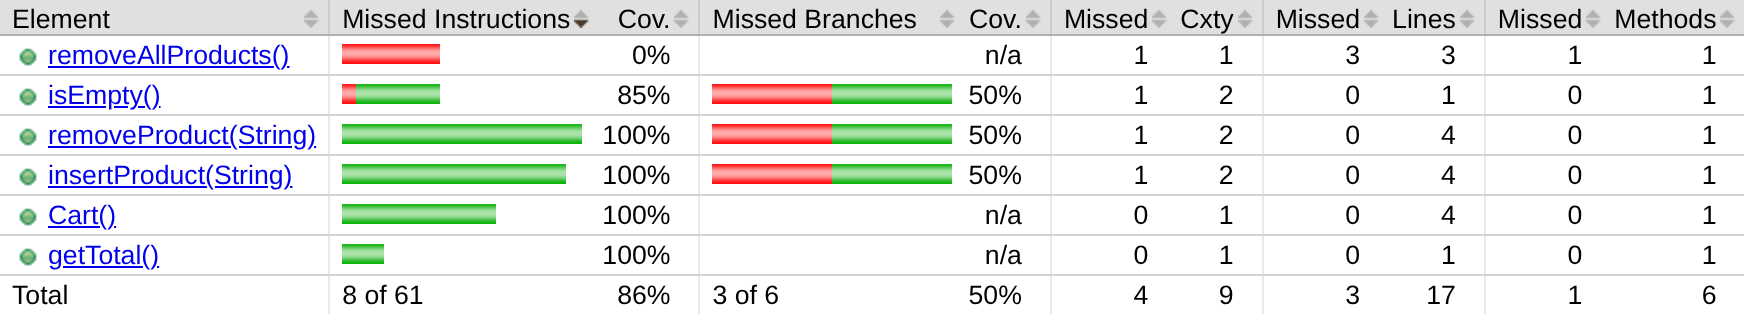
\includegraphics[width=0.92\linewidth]{jacoco_cart_metodi_3test}
\end{center}

E colora il sorgente, come fa IntelliJ: in \textbf{verde} le righe eseguite, in \textbf{rosso} quelle non eseguite, in
\textbf{giallo} quelle eseguite solo in parte. Il rombo a sinistra segnala una riga con dei rami; è giallo se solo una
parte dei rami è stata percorsa (passandoci sopra con il mouse il resoconto dice quanti: «1 of 2 branches missed»).

\Needspace{26\baselineskip}
\begin{center}
  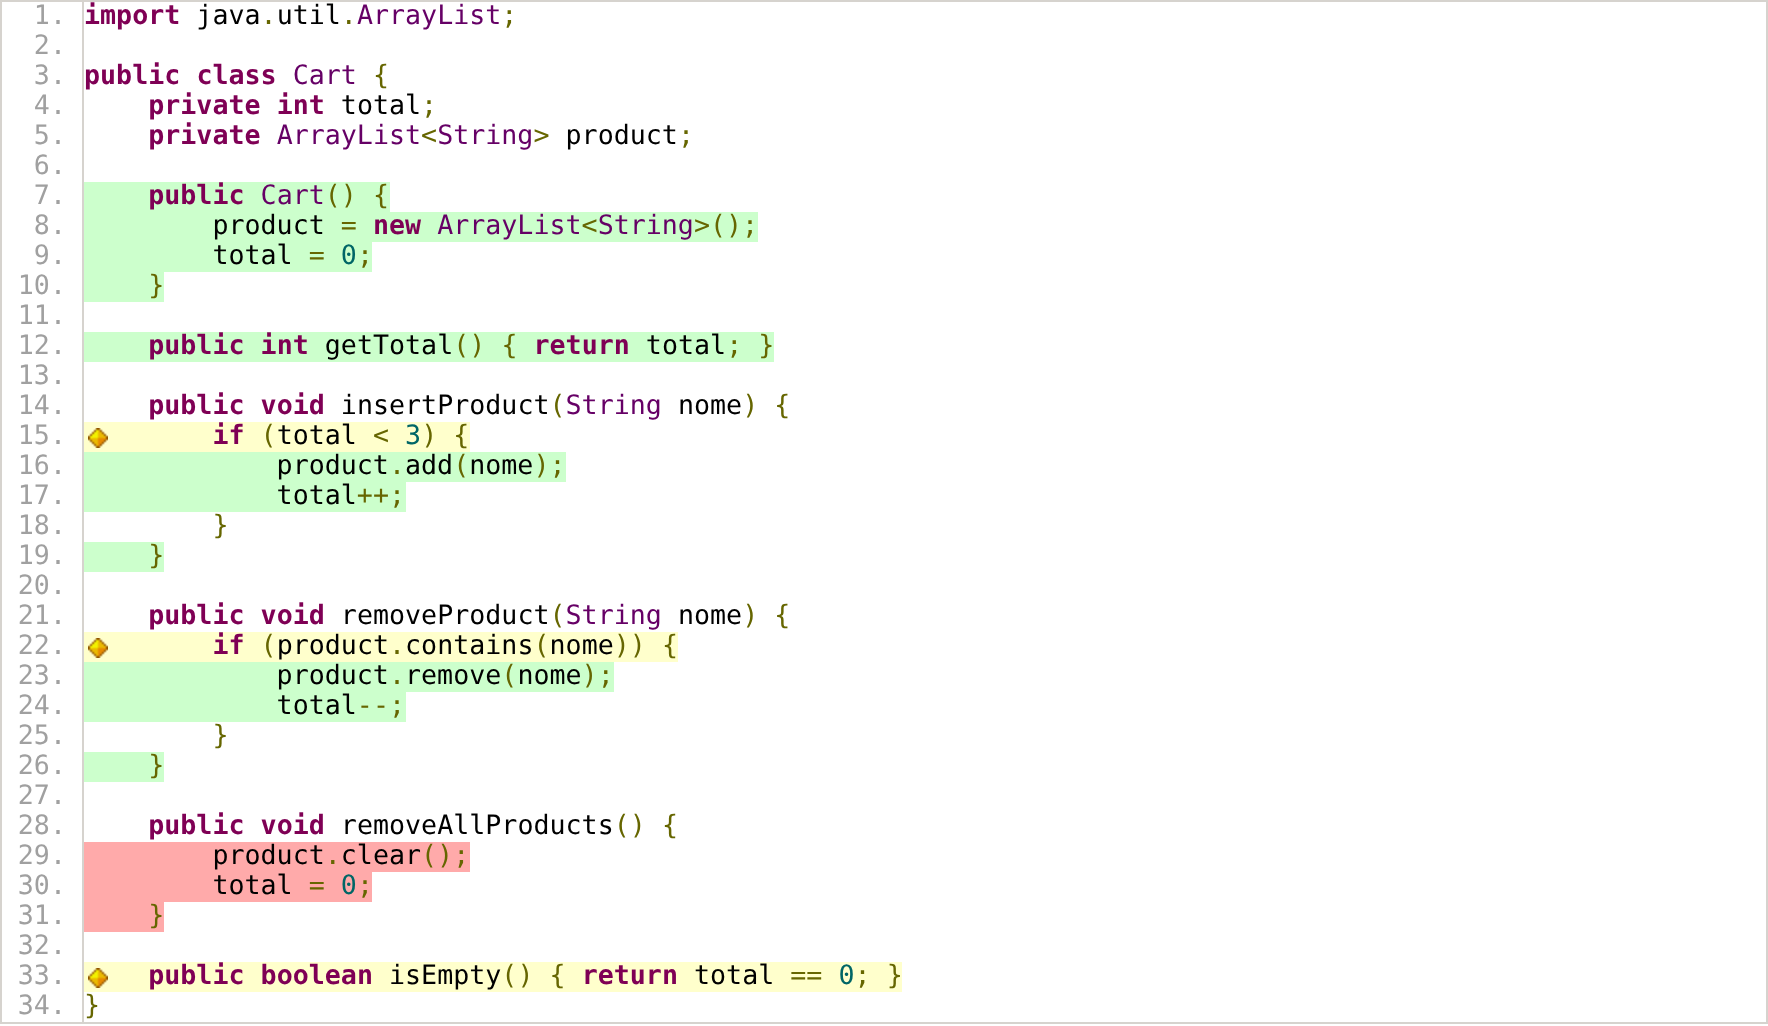
\includegraphics[width=0.78\linewidth]{jacoco_cart_sorgente_3test}
\end{center}

Il comportamento di JaCoCo, come spiegano le slide, è questo: a livello di \textbf{bytecode} la copertura di ogni
blocco è booleana (coperto o no); proiettata sul sorgente, ogni riga riceve un valore frazionario: 1 se tutti i blocchi
generati dalla riga sono stati coperti, un valore fra 0 e 1 se solo alcuni, 0 se nessuno. Le righe che non generano
bytecode (commenti, righe vuote, molte parentesi) non hanno copertura. Qui:

\begin{itemize}
  \item la riga 15 (\texttt{if (total < 3)}) è gialla: la condizione è stata vera, mai falsa (il carrello non è mai
        stato pieno); idem la riga 22, perché si è rimosso solo un prodotto presente;
  \item la riga 33 è gialla anch'essa: \texttt{total == 0} diventa nel bytecode un salto condizionato, e
        \texttt{isEmpty()} è stata chiamata solo su un carrello vuoto;
  \item le righe 29--31 sono rosse: nessun test chiama \texttt{removeAllProducts()}.
\end{itemize}

Nelle slide IntelliJ riporta per la stessa classe 5 metodi su 6 (83\%), 11 righe su 13 (84\%) e 2 rami su 4 (50\%).
JaCoCo conta 17 righe e 6 rami: considera righe anche le graffe di chiusura dei metodi \texttt{void} (vi sta il
\texttt{return} implicito) e conta come decisione anche il \texttt{total == 0}. Strumenti diversi contano in modo
diverso; il quadro però è lo stesso.

% ------------------------------------------------------------
\subsection{Test guidati dalla copertura}

Osservare il codice non eseguito porta a scrivere nuovi casi di test, fino a eseguire tutto il codice disponibile.
Mancano il caso del carrello pieno, la rimozione di un prodotto che non è nel carrello e la rimozione di tutti i
prodotti. Ecco i quattro test aggiunti nelle slide:

\Needspace{36\baselineskip}
\begin{lstlisting}[style=java, name=CartTest.java, firstnumber=42]
    @Test
    public void testRemoveAllProducts() {
        cart.insertProduct("prodotto1");
        cart.insertProduct("prodotto2");
        cart.removeAllProducts();
        assertTrue("Doveva essere vuoto", cart.isEmpty());
    }

    @Test
    public void testInsertMultipleProducts() {
        cart.insertProduct("prodotto1");
        cart.insertProduct("prodotto1");
        cart.removeProduct("prodotto1");
        assertEquals("Errore nel totale", 1, cart.getTotal());
    }

    @Test
    public void testRemoveProductNotInCart() {
        cart.insertProduct("prodotto1");
        cart.removeProduct("prodotto2");
        assertEquals("Non doveva essere rimosso", 1, cart.getTotal());
    }

    @Test
    public void testInsertMoreThanThreeProducts() {
        cart.insertProduct("prodotto1");
        cart.insertProduct("prodotto2");
        cart.insertProduct("prodotto3");
        cart.insertProduct("prodotto4");
        assertEquals("Errore nel totale", 3, cart.getTotal());
    }
\end{lstlisting}

\Needspace{24\baselineskip}
\begin{lstlisting}[style=shell, name=Terminale]
$ mvn test
...
[INFO] Running CartTest
[INFO] Tests run: 7, Failures: 0, Errors: 0, Skipped: 0, Time elapsed: 0.059 s -- in CartTest
[INFO]
[INFO] Results:
[INFO]
[INFO] Tests run: 7, Failures: 0, Errors: 0, Skipped: 0
...
[INFO] BUILD SUCCESS
...
$ cat target/site/jacoco/jacoco.csv
GROUP,PACKAGE,CLASS,INSTRUCTION_MISSED,INSTRUCTION_COVERED,BRANCH_MISSED,BRANCH_COVERED,LINE_MISSED,LINE_COVERED,COMPLEXITY_MISSED,COMPLEXITY_COVERED,METHOD_MISSED,METHOD_COVERED
carrello,default,Cart,1,60,1,5,0,17,1,8,0,6
\end{lstlisting}

Ora tutte le 17 righe e tutti i 6 metodi sono coperti; i rami, però, sono 5 su 6. Il resoconto mostra quale manca:

\Needspace{26\baselineskip}
\begin{center}
  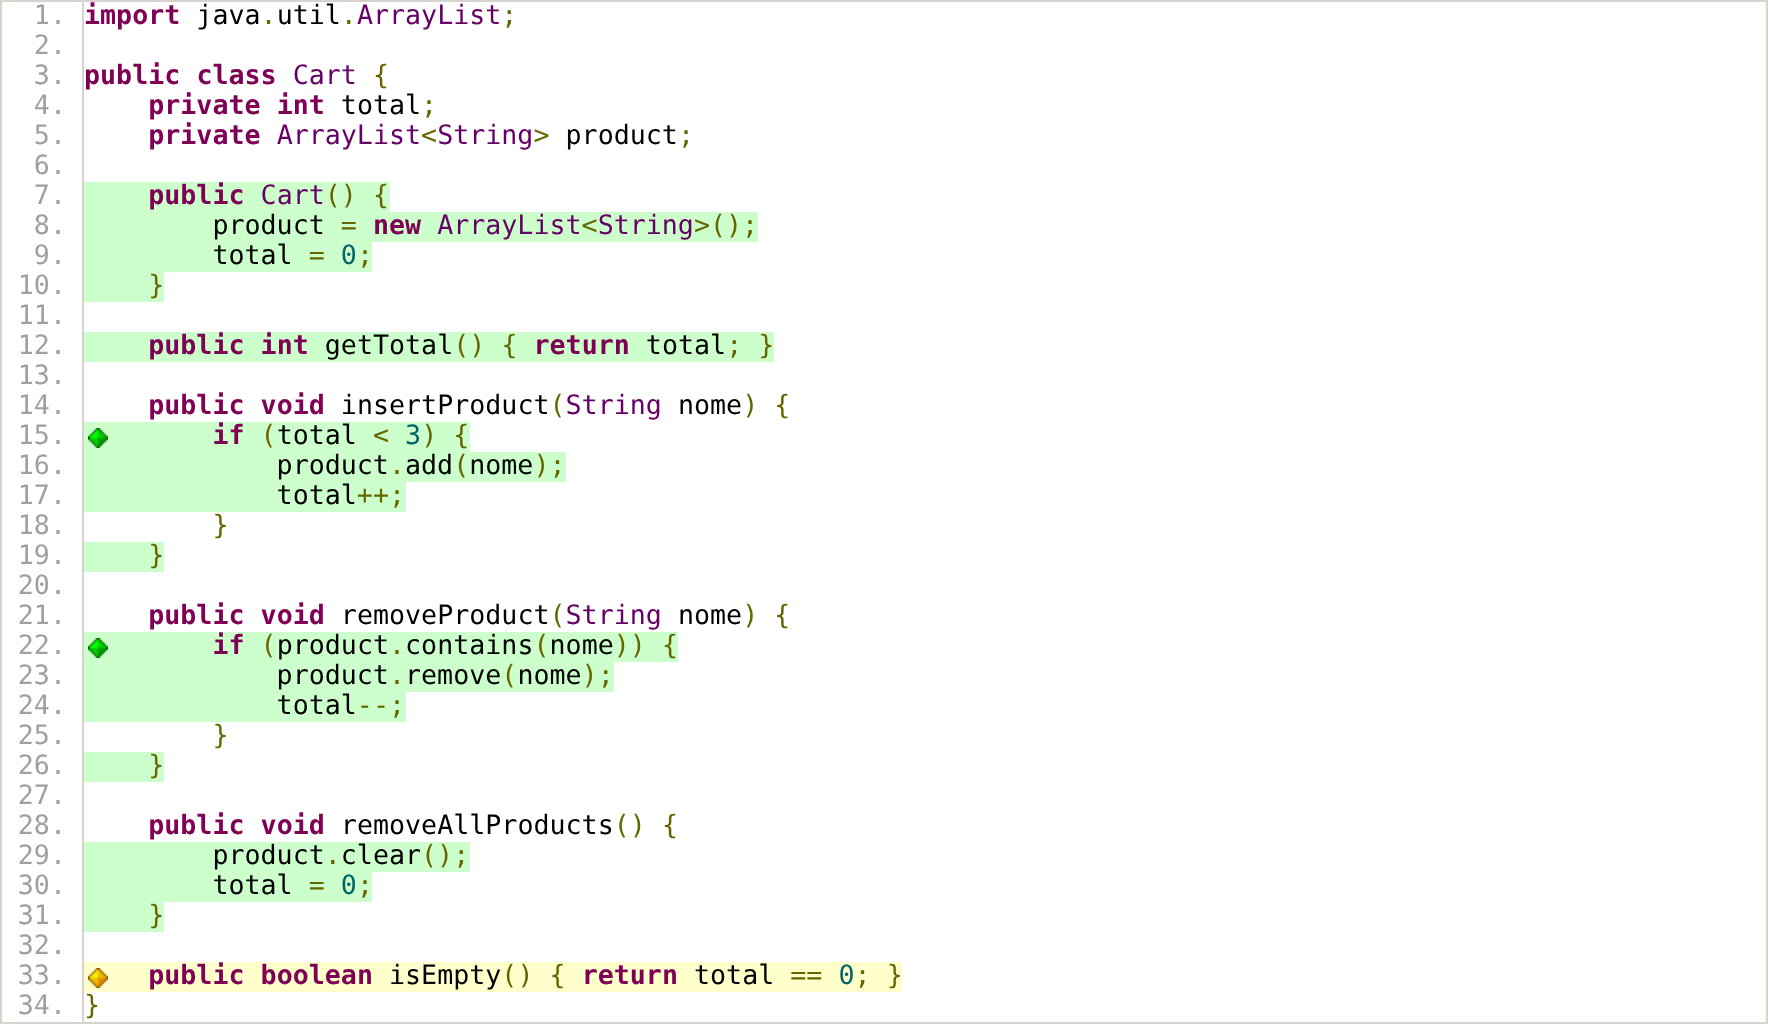
\includegraphics[width=0.78\linewidth]{jacoco_cart_sorgente_7test}
\end{center}

È ancora la riga 33: \texttt{isEmpty()} non è mai stata chiamata su un carrello \textbf{pieno}, quindi
\texttt{total == 0} non è mai stata falsa. Il 100\% delle righe non garantisce il 100\% dei rami: la copertura delle
istruzioni è un criterio debole, proprio come dice la teoria. Basterebbe un test che inserisce un prodotto e verifica
\texttt{assertFalse(cart.isEmpty())}.

% ------------------------------------------------------------
\subsection{Trovare i difetti}

Per vedere se i test trovano i difetti, le slide ne introducono due. Nel primo il limite del carrello è stato
impostato a 2 invece che a 3 (\texttt{if (total < 2)}):

\Needspace{26\baselineskip}
\begin{lstlisting}[style=shell, name=Terminale, deletekeywords={java}]
$ mvn test
...
[INFO] -------------------------------------------------------
[INFO]  T E S T S
[INFO] -------------------------------------------------------
[INFO] Running CartTest
[ERROR] Tests run: 7, Failures: 1, Errors: 0, Skipped: 0, Time elapsed: 0.054 s <<< FAILURE! -- in CartTest
[ERROR] CartTest.testInsertMoreThanThreeProducts -- Time elapsed: 0.007 s <<< FAILURE!
java.lang.AssertionError: Errore nel totale expected:<3> but was:<2>
    at org.junit.Assert.fail(Assert.java:89)
    at org.junit.Assert.failNotEquals(Assert.java:835)
    at org.junit.Assert.assertEquals(Assert.java:647)
    at CartTest.testInsertMoreThanThreeProducts(CartTest.java:71)
    at java.base/java.lang.reflect.Method.invoke(Method.java:580)

[INFO]
[INFO] Results:
[INFO]
[ERROR] Failures:
[ERROR]   CartTest.testInsertMoreThanThreeProducts:71 Errore nel totale expected:<3> but was:<2>
[INFO]
[ERROR] Tests run: 7, Failures: 1, Errors: 0, Skipped: 0
[INFO]
[INFO] ------------------------------------------------------------------------
[INFO] BUILD FAILURE
\end{lstlisting}

\Needspace{30\baselineskip}
Nel secondo il \texttt{total--} è finito per sbaglio fuori dall'\texttt{if} di \texttt{removeProduct}:

\begin{lstlisting}[style=java, name=Cart.java, firstnumber=21]
    public void removeProduct(String nome) {
        if (product.contains(nome)) {
            product.remove(nome);
        }
        total--;
    }
\end{lstlisting}

\begin{lstlisting}[style=shell, name=Terminale, deletekeywords={java}]
$ mvn test
...
[INFO] Running CartTest
[ERROR] Tests run: 7, Failures: 1, Errors: 0, Skipped: 0, Time elapsed: 0.050 s <<< FAILURE! -- in CartTest
[ERROR] CartTest.testRemoveProductNotInCart -- Time elapsed: 0.011 s <<< FAILURE!
java.lang.AssertionError: Non doveva essere rimosso expected:<1> but was:<0>
...
[ERROR] Failures:
[ERROR]   CartTest.testRemoveProductNotInCart:62 Non doveva essere rimosso expected:<1> but was:<0>
[INFO]
[ERROR] Tests run: 7, Failures: 1, Errors: 0, Skipped: 0
...
[INFO] BUILD FAILURE
\end{lstlisting}

Entrambi i difetti vengono trovati, e il messaggio di ogni asserzione dice subito quale comportamento è sbagliato. Ma li
trovano proprio i test aggiunti guardando la copertura. Con i soli tre test iniziali, entrambe le versioni difettose
superano il collaudo:

\begin{lstlisting}[style=shell, name=Terminale]
$ mvn test
...
[INFO] Running CartTest
[INFO] Tests run: 3, Failures: 0, Errors: 0, Skipped: 0, Time elapsed: 0.041 s -- in CartTest
[INFO]
[INFO] Results:
[INFO]
[INFO] Tests run: 3, Failures: 0, Errors: 0, Skipped: 0
...
[INFO] BUILD SUCCESS
\end{lstlisting}

(È l'esecuzione con il limite a 2; con il \texttt{total--} fuori posto il risultato è identico.) Le righe sbagliate,
del resto, erano proprio quelle che la copertura segnalava: la 15 gialla e la 22 gialla.

% ============================================================
\section{Test in isolamento e test di integrazione}

Il test di unità, a rigore, si può applicare solo a pezzi di software completamente \textbf{isolati}: dal resto del
software (le altre classi, le librerie), da altro software (il sistema operativo), da altre risorse (database, file,
rete). Un modulo \textbf{non} si può testare in isolamento se comunica con un database o in rete, se comunica con altri
moduli non ancora testati, se modifica database, file o altre sorgenti di dati, se non può essere eseguito in parallelo
con altri casi di test.

Le soluzioni concettuali sono due:

\begin{enumerate}
  \item \textbf{supporre corretti} tutti i moduli chiamati dal modulo sotto test e valide tutte le risorse a cui accede;
  \item \textbf{sostituire} tutti i moduli chiamati e le risorse usate con versioni fittizie e semplificate, la cui
        correttezza è garantita per costruzione.
\end{enumerate}

La prima è comoda ma rischiosa: un malfunzionamento osservato potrebbe venire da un modulo chiamato. La seconda è la
strada dei \textbf{driver} e degli \textbf{stub}.

% ------------------------------------------------------------
\subsection{Driver e stub}

Per testare un modulo «non terminale», cioè un modulo che a sua volta ne chiama altri, servono due tipi di moduli
ausiliari:

\begin{itemize}
  \item i \textbf{driver} invocano l'unità sotto test, passandole i valori del caso di test;
  \item gli \textbf{stub} vengono invocati dall'unità sotto test ed emulano la funzione chiamata nel caso di test
        richiesto, rispettandone la specifica; quando la funzione vera sarà realizzata e testata, prenderà il posto
        dello stub.
\end{itemize}

\begin{center}
\begin{tikzpicture}[
    mod/.style={rectangle, draw=#1!75!black, fill=#1!18, line width=0.7pt, font=\scriptsize,
                minimum width=1.5cm, minimum height=0.55cm},
    lab/.style={font=\scriptsize\itshape, anchor=west, text=black!75}]
  \node[mod=swred]   (main) at (0,0)        {\texttt{main}};
  \node[mod=swgreen] (a)    at (0,-1.1)     {A};
  \node[mod=swteal]  (d)    at (-1.1,-2.25) {D\,$'$};
  \node[mod=swteal]  (e)    at (1.1,-2.25)  {E\,$'$};
  \draw[tarco] (main) -- (a);
  \draw[tarco] (a) -- (d);
  \draw[tarco] (a) -- (e);
  \node[lab] (ld) at (3.0,0)     {driver};
  \node[lab] (la) at (3.0,-1.1)  {unità sotto test};
  \node[lab] (ls) at (3.0,-2.25) {stub};
  \draw[-{Stealth[length=1.6mm]}, draw=black!50] (ld.west) -- (main.east);
  \draw[-{Stealth[length=1.6mm]}, draw=black!50] (la.west) -- (a.east);
  \draw[-{Stealth[length=1.6mm]}, draw=black!50] (ls.west) -- (e.east);
\end{tikzpicture}
\end{center}

Il \textbf{driver} deve sostituire completamente il modulo (o i moduli) che chiamano quello da testare; un metodo di
test di JUnit è proprio un driver. Deve impostare tutti i valori delle risorse e delle sorgenti di dati usate dal modulo
da testare, costruire (nei linguaggi a oggetti) l'oggetto di cui si testa il metodo, e infine avviare il metodo.

Lo \textbf{stub} è una funzione fittizia, \textbf{corretta per ipotesi}. L'esempio delle slide: si vuole testare una
funzione \texttt{prod\_scal(v1, v2)} che calcola il prodotto scalare di due vettori invocando una funzione
\texttt{product(a, b)} non ancora realizzata. Nel driver si eseguono alcuni casi di test, per esempio
\texttt{prod\_scal([2,4], [4,7])}, e lo stub di \texttt{product} risponde solo a quelli:

\Needspace{20\baselineskip}
\begin{lstlisting}[style=java, name=ProdottoScalare.java]
public class ProdottoScalare {
    public static int prod_scal(int[] v1, int[] v2) {
        int somma = 0;
        for (int i = 0; i < v1.length; i++)
            somma += product(v1[i], v2[i]);
        return somma;
    }

    // STUB: product non e' ancora stata realizzata
    static int product(int a, int b) {
        if (a == 2 && b == 4) return 8;
        if (a == 4 && b == 7) return 28;
    }
}
\end{lstlisting}

\begin{lstlisting}[style=shell, name=Terminale]
$ javac ProdottoScalare.java
ProdottoScalare.java:13: error: missing return statement
    }
    ^
1 error
\end{lstlisting}

Scritto così, come nelle slide, lo stub \textbf{non compila}: Java pretende che un metodo \texttt{int} restituisca un
valore lungo ogni cammino, e quando nessuno dei due \texttt{if} è vero manca il \texttt{return}. La soluzione naturale è
far fallire rumorosamente lo stub nei casi che non prevede: se un driver gli chiede qualcosa di inatteso, lo si scopre
subito.

\begin{lstlisting}[style=java, name=ProdottoScalare.java, firstnumber=10]
    static int product(int a, int b) {
        if (a == 2 && b == 4) return 8;
        if (a == 4 && b == 7) return 28;
        throw new IllegalStateException("caso non previsto dallo stub: " + a + ", " + b);
    }
\end{lstlisting}

\Needspace{12\baselineskip}
E il driver è un test JUnit: $2 \cdot 4 + 4 \cdot 7 = 36$.

\begin{lstlisting}[style=java, name=ProdottoScalareTest.java]
import static org.junit.Assert.assertEquals;

import org.junit.Test;

// Il driver: prepara i dati, chiama l'unita' sotto test, controlla il risultato
public class ProdottoScalareTest {

    @Test
    public void testProdScal() {
        assertEquals(36, ProdottoScalare.prod_scal(new int[] {2, 4}, new int[] {4, 7}));
    }
}
\end{lstlisting}

\Needspace{14\baselineskip}
\begin{lstlisting}[style=shell, name=Terminale]
$ mvn test -Dtest=ProdottoScalareTest
...
[INFO] Running ProdottoScalareTest
[INFO] Tests run: 1, Failures: 0, Errors: 0, Skipped: 0, Time elapsed: 0.043 s -- in ProdottoScalareTest
[INFO]
[INFO] Results:
[INFO]
[INFO] Tests run: 1, Failures: 0, Errors: 0, Skipped: 0
...
[INFO] BUILD SUCCESS
\end{lstlisting}

(L'opzione \texttt{-Dtest=} di Surefire esegue solo la classe di test indicata, o più classi separate da virgole.) La
correttezza dello stub è data per ipotesi; per scriverlo, ovviamente, bisogna sapere con precisione come il modulo
sotto test userà la funzione che manca.

Più in generale, il termine \textbf{stub} indica un metodo fittizio, non ancora implementato o la cui implementazione è
volutamente incompleta: spesso gli stub stanno nel codice solo per ricordare i metodi ancora da scrivere, o per poter
compilare il prima possibile. Uno stub riproduce il comportamento del modulo che sostituisce \textbf{solo nei casi di
test previsti dai driver}; si può scrivere conoscendo il modulo da emulare solo a scatola nera, e permette di testare un
modulo prima che siano costruiti quelli da cui dipende. Ha però un limite preciso:

\begin{itemize}
  \item uno stub sostituisce bene una \textbf{funzione} o un metodo: a ogni caso di test corrisponde un'istanza diversa
        dello stub, o un ramo diverso;
  \item uno stub \textbf{non} sostituisce bene una \textbf{classe}: non può gestire lo stato (i valori degli attributi)
        fra due chiamate, né il test di una sequenza di interazioni.
\end{itemize}

% ------------------------------------------------------------
\subsection{Il test di integrazione}

Dopo aver testato tutte le unità, serve il \textbf{test di integrazione}, per valutare se funzionano bene
\textbf{insieme}. Se \texttt{a} chiama \texttt{b} ed entrambi hanno superato i test di unità, la coppia potrebbe
comunque non superare tutti i test richiesti ad \texttt{a}: per esempio perché \texttt{a} chiama \texttt{b} con
combinazioni di input che chi ha testato \texttt{b} non aveva previsto. Per testare insieme \texttt{a} e \texttt{b}
possono bastare i test progettati per \texttt{a}: in pratica, nei test di \texttt{a} si mette il vero \texttt{b} al posto
del suo stub (o del suo mock).

Le strategie di integrazione sono tre, e si distinguono per il punto da cui si comincia:

\begin{itemize}
  \item \textbf{top-down}: si parte dall'alto (l'interfaccia utente), sostituendo con degli stub i livelli sottostanti;
        poi si scende, rimpiazzando gli stub con i moduli veri, che a loro volta useranno stub per i livelli inferiori;
  \item \textbf{bottom-up}: si parte dal basso (i livelli di accesso al database e alla rete), facendoli chiamare da
        driver; poi si sale, aggiungendo i livelli superiori sopra quelli già testati;
  \item \textbf{sandwich}: si combinano le due, procedendo dall'alto con gli stub e dal basso con i driver, fino a
        incontrarsi nel mezzo.
\end{itemize}

\begin{center}
\begin{tikzpicture}[
    liv/.style={rectangle, draw=black!75, fill=#1!12, line width=0.6pt, font=\tiny, align=center,
                minimum height=0.42cm, inner sep=1.5pt},
    liv/.default=swblue,
    aus/.style={rectangle, draw=#1!75!black, fill=#1!15, line width=0.5pt, font=\tiny,
                minimum width=0.62cm, minimum height=0.3cm, inner sep=1pt},
    ch/.style={-{Stealth[length=1.3mm]}, line width=0.45pt, draw=black!70},
    passo/.style={-{Stealth[length=2.4mm]}, line width=1pt, draw=swgray},
    tit/.style={font=\scriptsize\bfseries}]

  % --- top-down ---
  \begin{scope}[shift={(0,0)}]
    \node[tit] at (0,0.75) {Top-down};
    \node[liv, minimum width=2.3cm] (ui) at (0,0) {Interfaccia utente};
    \foreach \x/\n in {-0.75/a, 0/b, 0.75/c}
      { \node[aus=swteal] (s\n) at (\x,-0.62) {stub}; \draw[ch] (ui.south -| s\n) -- (s\n); }
    \draw[passo] (0,-0.95) -- (0,-1.5);
    \node[liv, minimum width=2.3cm] (ui2) at (0,-1.8) {Interfaccia utente};
    \node[liv=swgreen, minimum width=2.3cm] (fn2) at (0,-2.45) {Livello funzionale};
    \foreach \x in {-0.75, 0, 0.75} \draw[ch] (\x,-2.01) -- (\x,-2.24);
    \foreach \x/\n in {-0.75/a, 0/b, 0.75/c}
      { \node[aus=swteal] (t\n) at (\x,-3.07) {stub}; \draw[ch] (fn2.south -| t\n) -- (t\n); }
  \end{scope}

  % --- bottom-up ---
  \begin{scope}[shift={(4.4,0)}]
    \node[tit] at (0,0.75) {Bottom-up};
    \foreach \x/\n in {-0.82/a, 0/b, 0.82/c} \node[aus=swred] (d\n) at (\x,0.25) {driver};
    \node[liv=sworange, minimum width=1.12cm] (db) at (-0.59,-0.4) {Database};
    \node[liv=sworange, minimum width=1.12cm] (nw) at (0.59,-0.4) {Rete};
    \foreach \x in {-0.82, 0, 0.82} \draw[ch] (\x,0.1) -- (\x,-0.19);
    \draw[passo] (0,-0.75) -- (0,-1.3);
    \foreach \x/\n in {-0.82/a, 0/b, 0.82/c} \node[aus=swred] (e\n) at (\x,-1.55) {driver};
    \node[liv=swgreen, minimum width=2.3cm] (fn) at (0,-2.15) {Livello funzionale};
    \foreach \x in {-0.82, 0, 0.82} \draw[ch] (\x,-1.7) -- (\x,-1.94);
    \node[liv=sworange, minimum width=1.12cm] (db2) at (-0.59,-2.85) {Database};
    \node[liv=sworange, minimum width=1.12cm] (nw2) at (0.59,-2.85) {Rete};
    \foreach \x in {-0.75, 0, 0.75} \draw[ch] (\x,-2.36) -- (\x,-2.64);
  \end{scope}

  % --- sandwich ---
  \begin{scope}[shift={(8.8,0)}]
    \node[tit] at (0,0.75) {Sandwich};
    \node[liv, minimum width=2.3cm] (uis) at (0,0) {Interfaccia utente};
    \foreach \x/\n in {-0.75/a, 0/b, 0.75/c}
      { \node[aus=swteal] (u\n) at (\x,-0.62) {stub}; \draw[ch] (uis.south -| u\n) -- (u\n); }
    \draw[passo] (0,-0.95) -- (0,-1.3);
    \foreach \x/\n in {-0.82/a, 0/b, 0.82/c} \node[aus=swred] (f\n) at (\x,-1.55) {driver};
    \node[liv=sworange, minimum width=1.12cm] (dbs) at (-0.59,-2.2) {Database};
    \node[liv=sworange, minimum width=1.12cm] (nws) at (0.59,-2.2) {Rete};
    \foreach \x in {-0.82, 0, 0.82} \draw[ch] (\x,-1.7) -- (\x,-1.99);
  \end{scope}

  % --- sistema integrato ---
  \begin{scope}[shift={(4.4,-4.3)}]
    \node[liv, minimum width=2.3cm] (uif) at (0,0) {Interfaccia utente};
    \node[liv=swgreen, minimum width=2.3cm] (fnf) at (0,-0.65) {Livello funzionale};
    \foreach \x in {-0.75, 0, 0.75} \draw[ch] (\x,-0.21) -- (\x,-0.44);
    \node[liv=sworange, minimum width=1.12cm] (dbf) at (-0.59,-1.35) {Database};
    \node[liv=sworange, minimum width=1.12cm] (nwf) at (0.59,-1.35) {Rete};
    \foreach \x in {-0.75, 0, 0.75} \draw[ch] (\x,-0.86) -- (\x,-1.14);
    \node[font=\scriptsize, align=right, anchor=east] at (-1.4,-0.65) {sistema\\completamente\\integrato};
  \end{scope}

  \draw[passo] (0.6,-3.4) -- (3.0,-4.15);
  \draw[passo] (4.4,-3.2) -- (4.4,-3.95);
  \draw[passo] (8.6,-2.55) -- (5.8,-4.15);
\end{tikzpicture}
\end{center}

% ------------------------------------------------------------
\subsection{Un esempio: il calendario}

L'esempio delle slide è la classe \texttt{Calendario} che risolve il problema del giorno della settimana (lo stesso
della sezione sulle classi di equivalenza), divisa in cinque metodi statici:

\begin{itemize}
  \item \texttt{main} legge dalla riga di comando giorno, mese (come stringa) e anno;
  \item \texttt{giornoDellaSettimana} converte il mese in un intero, controlla che la data sia valida e, se lo è, chiama
        \texttt{calend};
  \item \texttt{valida} controlla se la data è valida;
  \item \texttt{calend} calcola il giorno della settimana (come intero);
  \item \texttt{convert} converte il giorno della settimana in stringa.
\end{itemize}

\begin{center}
\begin{tikzpicture}[
    met/.style={rectangle, rounded corners=2pt, draw=swblue!75!black, fill=swblue!8, line width=0.6pt,
                font=\scriptsize\ttfamily, inner sep=3pt}]
  \node[met] (main) at (0,0)        {main(...)};
  \node[met] (gds)  at (0,-1.1)     {giornoDellaSettimana(...)};
  \node[met] (cal)  at (-1.3,-2.2)  {calend(...)};
  \node[met] (val)  at (1.3,-2.2)   {valida(...)};
  \node[met] (conv) at (-1.3,-3.3)  {convert(...)};
  \draw[tarco] (main) -- (gds);
  \draw[tarco] (gds) -- (cal);
  \draw[tarco] (gds) -- (val);
  \draw[tarco] (cal) -- (conv);
  \node[draw=q9!75!black, line width=0.7pt, rounded corners=3pt, inner sep=8pt,
        fit=(main)(gds)(cal)(val)(conv)] (cl) {};
  \node[anchor=south west, font=\scriptsize\bfseries, fill=white, inner sep=2pt]
    at ([xshift=6pt, yshift=-5pt]cl.north west) {Calendario};
\end{tikzpicture}
\end{center}

\Needspace{20\baselineskip}
Ecco il codice delle slide, ricomposto in un unico file (nelle slide è distribuito su cinque pagine):

\begin{lstlisting}[style=java, name=Calendario.java]
public class Calendario {

    public static String main(String[] args) {
        if (args.length == 3) {
            int giorno = Integer.parseInt(args[0]);
            String mese = args[1];
            int anno = Integer.parseInt(args[2]);
            String giornoDS = new String(giornoDellaSettimana(giorno, mese, anno));
            System.out.println(giornoDS);
            return giornoDS;
        }
        else
            return "";
    }

    public static String giornoDellaSettimana(int d, String ms, int a) {
        int m = 0;
        if (ms.equals("gennaio")) m = 1;
        else if (ms.equals("febbraio")) m = 2;
        else if (ms.equals("marzo")) m = 3;
        else if (ms.equals("aprile")) m = 4;
        else if (ms.equals("maggio")) m = 5;
        else if (ms.equals("giugno")) m = 6;
        else if (ms.equals("luglio")) m = 7;
        else if (ms.equals("agosto")) m = 8;
        else if (ms.equals("settembre")) m = 9;
        else if (ms.equals("ottobre")) m = 10;
        else if (ms.equals("novembre")) m = 11;
        else if (ms.equals("dicembre")) m = 12;
        if ((m > 0) && valida(d, m, a))
            return calend(d, m, a);
        else
            return "Errore";
    }

    public static boolean valida(int d, int m, int a) {
        if (d < 1 || d > 31 || m == 0 || a <= 1582)
            return false;
        Boolean bisestile = (a % 4 == 0);
        if (bisestile && a % 100 == 0 && a % 400 != 0)
            bisestile = false;
        if ((m == 2 && d > 29) || (m == 2 && d == 29 && !bisestile))
            return false;
        if ((m == 4 || m == 6 || m == 9 || m == 11) && d > 30)
            return false;
        return true;
    }

    public static String calend(int d, int m, int a) {
        if (m <= 2) {
            m = m + 12;
            a--;
        };
        int f1 = a / 4;
        int f2 = a / 100;
        int f3 = a / 400;
        int f4 = (int) (2 * m + (.6 * (m + 1)));
        int f5 = a + d + 1;
        int x = f1 - f2 + f3 + f4 + f5;
        int k = x / 7;
        int n = x - k * 7;
        return convert(n);
    }

    public static String convert(int n) {
        if (n == 1) return "Lunedi";
        else if (n == 2) return "Martedi";
        else if (n == 3) return "Mercoledi";
        else if (n == 4) return "Giovedi";
        else if (n == 5) return "Venerdi";
        else if (n == 6) return "Sabato";
        else if (n == 0) return "Domenica";
        else return "Errore";
    }
}
\end{lstlisting}

\texttt{calend} applica una variante della formula di Zeller: i mesi di gennaio e febbraio contano come mesi 13 e 14
dell'anno precedente, così il giorno in più dell'anno bisestile cade alla fine; \texttt{f1 - f2 + f3} conta i giorni
bisestili accumulati con le regole del calendario gregoriano, e il resto della divisione per 7 dà il giorno della
settimana (0 è domenica). Che il risultato sia giusto lo conferma l'oracolo software della sezione sui valori limite:
nessun giorno della settimana sbagliato su più di duecentomila date. Il difetto di \texttt{valida} con l'anno 1582,
trovato proprio dai valori limite, resta anche qui.

\Needspace{16\baselineskip}
\begin{warningbox}{{Un main che restituisce String}}
  Nelle slide \texttt{main} restituisce la stringa calcolata, così i test possono controllarla. Ma con quella firma non
  è più il punto di ingresso del programma:

  \begin{lstlisting}[style=shell, name=Terminale]
$ javac Calendario.java
$ java Calendario 24 aprile 2011
Error: Main method must return a value of type void in class Calendario, please
define the main method as:
   public static void main(String[] args)
\end{lstlisting}

  La classe compila (\texttt{main} è un nome di metodo come un altro), ma la JVM si rifiuta di avviarla. In un programma
  vero il calcolo starebbe in un metodo a parte, da testare, e \texttt{public static void main} si limiterebbe a
  chiamarlo e a stampare il risultato.
\end{warningbox}

\subsubsection*{Integrazione bottom-up}

Dal basso: prima \texttt{convert}, che non chiama nessuno; poi \texttt{calend}, che chiama \texttt{convert} (già
testata); poi \texttt{valida}, poi \texttt{giornoDellaSettimana} e infine \texttt{main}. Non serve nessuno stub: ogni
metodo usa solo metodi già testati, e i driver sono i metodi di test.

\Needspace{38\baselineskip}
\begin{lstlisting}[style=java, name=CalendarioTest.java]
import static org.junit.Assert.*;

import org.junit.Test;

// Test bottom-up: dalle unita' foglia (convert) fino a main
public class CalendarioTest {

    @Test
    public void testConvert1() {
        assertEquals("Domenica", Calendario.convert(0));
    }

    @Test
    public void testCalend1() {
        assertEquals("Domenica", Calendario.calend(24, 4, 2011));
    }

    @Test
    public void testValida1() {
        assertTrue(Calendario.valida(24, 4, 2011));
    }

    @Test
    public void testGiornoDellaSettimana1() {
        assertEquals("Domenica", Calendario.giornoDellaSettimana(24, "aprile", 2011));
    }

    @Test
    public void testMain1() {
        String a[] = new String[3];
        a[0] = "24";
        a[1] = "aprile";
        a[2] = "2011";
        assertEquals("Domenica", Calendario.main(a));
    }
}
\end{lstlisting}

\Needspace{16\baselineskip}
\begin{lstlisting}[style=shell, name=Terminale]
$ mvn test -Dtest=CalendarioTest
...
[INFO] Running CalendarioTest
Domenica
[INFO] Tests run: 5, Failures: 0, Errors: 0, Skipped: 0, Time elapsed: 0.059 s -- in CalendarioTest
[INFO]
[INFO] Results:
[INFO]
[INFO] Tests run: 5, Failures: 0, Errors: 0, Skipped: 0
...
[INFO] BUILD SUCCESS
\end{lstlisting}

Il 24 aprile 2011 era davvero una domenica (era Pasqua). La riga \texttt{Domenica} in mezzo al resoconto è la stampa
di \texttt{main}: ai test non dà fastidio, ma finisce mescolata ai messaggi di Maven.

\subsubsection*{Integrazione top-down}

Dall'alto: per testare \texttt{main} basta uno stub di \texttt{giornoDellaSettimana} che risponda ai due casi di test
previsti, la data del 24 aprile 2011 (TC1) e quella, non valida, del 32 aprile 2011 (TC2). Lo stub delle slide è questo:

\begin{lstlisting}[style=java, name=Calendario.java, firstnumber=16]
    public static String giornoDellaSettimana(int d, String ms, int a) {
        //STUB
        if (d == 24 && ms.equals("aprile") && a == 2011)
            return "Domenica"; //TC1
        else if (d == 32 && ms.equals("aprile") && a == 2011)
            return ""; //TC2
        return "";
    }
\end{lstlisting}

\Needspace{14\baselineskip}
I casi di test di \texttt{main}, progettati sulla specifica, si aspettano «Domenica» per la data valida ed «Errore» per
quella non valida:

\begin{lstlisting}[style=java, name=CalendarioMainTest.java]
import static org.junit.Assert.*;

import org.junit.Test;

// Casi di test di main, progettati sulla specifica
public class CalendarioMainTest {

    @Test
    public void testMainTC1() {
        assertEquals("Domenica", Calendario.main(new String[] {"24", "aprile", "2011"}));
    }

    @Test
    public void testMainTC2() {
        assertEquals("Errore", Calendario.main(new String[] {"32", "aprile", "2011"}));
    }
}
\end{lstlisting}

\Needspace{26\baselineskip}
Prima dell'esecuzione si è messa in \texttt{src/main/java}, al posto di \texttt{Calendario.java}, la versione con lo
stub:

\begin{lstlisting}[style=shell, name=Terminale, deletekeywords={java}]
$ mvn test -Dtest=CalendarioMainTest
...
[INFO] Running CalendarioMainTest
Domenica

[ERROR] Tests run: 2, Failures: 1, Errors: 0, Skipped: 0, Time elapsed: 0.076 s <<< FAILURE! -- in CalendarioMainTest
[ERROR] CalendarioMainTest.testMainTC2 -- Time elapsed: 0.011 s <<< FAILURE!
org.junit.ComparisonFailure: expected:<[Errore]> but was:<[]>
    at org.junit.Assert.assertEquals(Assert.java:117)
    at org.junit.Assert.assertEquals(Assert.java:146)
    at CalendarioMainTest.testMainTC2(CalendarioMainTest.java:15)
    at java.base/java.lang.reflect.Method.invoke(Method.java:580)

[INFO]
[INFO] Results:
[INFO]
[ERROR] Failures:
[ERROR]   CalendarioMainTest.testMainTC2:15 expected:<[Errore]> but was:<[]>
[INFO]
[ERROR] Tests run: 2, Failures: 1, Errors: 0, Skipped: 0
...
[INFO] BUILD FAILURE
\end{lstlisting}

Il test TC2 fallisce, ma \texttt{main} non ha colpe: la vera \texttt{giornoDellaSettimana}, per una data non valida,
restituisce «Errore», mentre lo stub delle slide restituisce la stringa vuota (la riga vuota sotto «Domenica» è la sua
stampa). Uno stub che non rispetta la specifica del metodo che sostituisce produce \textbf{falsi allarmi}, o peggio
nasconde i difetti veri. Per i confronti fra stringhe JUnit~4 lancia una \texttt{ComparisonFailure} e mette fra
parentesi quadre la parte che differisce: qui tutta.

\Needspace{18\baselineskip}
Per testare \texttt{giornoDellaSettimana} servono invece gli stub di \texttt{calend} e di \texttt{valida}. Nelle slide
coprono anche un terzo caso, il 29 febbraio 2012:

\begin{lstlisting}[style=java, name=Calendario.java, firstnumber=36]
    public static boolean valida(int d, int m, int a) {
        //STUB
        if (d == 24 && m == 4 && a == 2011) return true;
        else if (d == 29 && m == 2 && a == 2012) return true;
        else if (d == 32 && m == 4 && a == 2011) return false;
        return false;
    }

    public static String calend(int d, int m, int a) {
        // STUB
        if (d == 24 && m == 4 && a == 2011) return "Domenica";
        else if (d == 29 && m == 2 && a == 2012) return "Lunedi";
        else return "";
    }
\end{lstlisting}

\Needspace{24\baselineskip}
\begin{lstlisting}[style=java, name=CalendarioGiornoTest.java]
import static org.junit.Assert.*;

import org.junit.Test;

// Casi di test di giornoDellaSettimana, progettati sulla specifica
public class CalendarioGiornoTest {

    @Test
    public void testTC1() {
        assertEquals("Domenica", Calendario.giornoDellaSettimana(24, "aprile", 2011));
    }

    @Test
    public void testTC2() {
        assertEquals("Mercoledi", Calendario.giornoDellaSettimana(29, "febbraio", 2012));
    }

    @Test
    public void testTC3() {
        assertEquals("Errore", Calendario.giornoDellaSettimana(32, "aprile", 2011));
    }
}
\end{lstlisting}

\Needspace{24\baselineskip}
\begin{lstlisting}[style=shell, name=Terminale, deletekeywords={java}]
$ mvn test -Dtest=CalendarioGiornoTest
...
[INFO] Running CalendarioGiornoTest
[ERROR] Tests run: 3, Failures: 1, Errors: 0, Skipped: 0, Time elapsed: 0.040 s <<< FAILURE! -- in CalendarioGiornoTest
[ERROR] CalendarioGiornoTest.testTC2 -- Time elapsed: 0.004 s <<< FAILURE!
org.junit.ComparisonFailure: expected:<[Mercol]edi> but was:<[Lun]edi>
    at org.junit.Assert.assertEquals(Assert.java:117)
    at org.junit.Assert.assertEquals(Assert.java:146)
    at CalendarioGiornoTest.testTC2(CalendarioGiornoTest.java:15)
    at java.base/java.lang.reflect.Method.invoke(Method.java:580)

[INFO]
[INFO] Results:
[INFO]
[ERROR] Failures:
[ERROR]   CalendarioGiornoTest.testTC2:15 expected:<[Mercol]edi> but was:<[Lun]edi>
[INFO]
[ERROR] Tests run: 3, Failures: 1, Errors: 0, Skipped: 0
...
[INFO] BUILD FAILURE
\end{lstlisting}

Di nuovo un falso allarme: il 29 febbraio 2012 era un \textbf{mercoledì}, non un lunedì come dice lo stub delle slide.
Chi scrive uno stub deve conoscere bene il comportamento atteso del modulo che emula: lo stub è «corretto per ipotesi»,
ma l'ipotesi va verificata. (Qui le parentesi quadre isolano la parte diversa delle due stringhe, \texttt{edi} è in
comune.)

\subsubsection*{L'integrazione}

Rimettendo al loro posto i metodi veri, gli stessi casi di test diventano test di integrazione:

\begin{lstlisting}[style=shell, name=Terminale, deletestring={[b]'}]
$ mvn test -Dtest='CalendarioMainTest,CalendarioGiornoTest'
...
[INFO] Running CalendarioGiornoTest
[INFO] Tests run: 3, Failures: 0, Errors: 0, Skipped: 0, Time elapsed: 0.043 s -- in CalendarioGiornoTest
[INFO] Running CalendarioMainTest
Domenica
Errore
[INFO] Tests run: 2, Failures: 0, Errors: 0, Skipped: 0, Time elapsed: 0.018 s -- in CalendarioMainTest
[INFO]
[INFO] Results:
[INFO]
[INFO] Tests run: 5, Failures: 0, Errors: 0, Skipped: 0
...
[INFO] BUILD SUCCESS
\end{lstlisting}

Tutti e cinque passano: i fallimenti di prima erano davvero colpa degli stub.

\subsubsection*{Altre strategie: il test in isolamento}

Si può anche partire da un modulo intermedio. Se per esempio \texttt{calend} fosse stato realizzato per primo (magari
per fare un prototipo, visto che è l'unico metodo la cui complessità viene da conoscenze astronomiche), servirebbero:

\begin{itemize}
  \item un \textbf{driver} che si comporti come \texttt{giornoDellaSettimana}: può essere il metodo di test JUnit già
        pensato per le strategie top-down e bottom-up;
  \item uno \textbf{stub} che faccia le veci di \texttt{convert} nei casi richiesti dal driver. (Le slide suggeriscono
        di riusare «lo stub pensato per il bottom-up», ma il bottom-up non usa stub: questo va scritto apposta.)
\end{itemize}

\subsubsection*{I limiti di stub e driver}

La tecnica ha dei problemi, soprattutto nei linguaggi a oggetti:

\begin{itemize}
  \item uno stub sostituisce facilmente solo un metodo \textbf{combinatorio}, senza stato: se il metodo legge o modifica
        gli attributi della classe, bisogna implementare altri metodi (stub o veri) che facciano quelle operazioni;
  \item ogni caso di test ha bisogno di uno stub diverso, e gli stub sostituiscono i metodi: prima di ogni test bisogna
        mettere lo stub al posto del metodo originale e ricompilare. È proprio quello che si è fatto qui sopra, copiando
        a mano una versione diversa di \texttt{Calendario.java} prima di ogni esecuzione: un pessimo supporto
        all'automazione;
  \item i driver si possono scrivere come casi di test JUnit, ma gli stub restano pezzi di codice scomodi, da usare o
        da ignorare a seconda del test.
\end{itemize}

Si può evitare di gestire stub espliciti, e scrivere un caso di test \textbf{interamente} dentro un metodo di test
JUnit? Sì: con i \textbf{test double} e i \textbf{mock object}.

% ============================================================
\section{Test double e mock object}

Un \textbf{test double} (una «controfigura», come quelle del cinema) è un'implementazione alternativa di un'interfaccia
o di una classe che nel test non si può usare: perché è troppo lenta; perché non è (ancora) disponibile, o dipende da
qualcosa che non lo è; perché è troppo difficile da istanziare e configurare per un test; perché compie operazioni
irreversibili; perché interagisce con risorse imprevedibili, come un generatore di numeri casuali o una connessione di
rete. Lo stub della sezione precedente è un caso particolare: il test double di una \textbf{funzione}. Per emulare con
precisione il comportamento di \textbf{classi} non ancora implementate si usano invece i \textbf{mock object}.

\dfn{Mock object}{
  Simulazione di un oggetto reale. Implementa l'interfaccia dell'oggetto da simulare e ha un comportamento proprio: può
  fornire risposte prefissate, come uno stub, e può \textbf{controllare} che l'oggetto che lo usa lo faccia
  correttamente.}

Perché l'oggetto sotto test lavori con il mock al posto dell'oggetto vero, bisogna poterglielo passare dall'esterno: è la
\textbf{Dependency Injection} del Capitolo~15, dove \texttt{AllarmeCaldo} riceveva nel test un \texttt{MeteoFinto} al
posto del servizio meteo vero. Per il test in isolamento e per quello di integrazione è fondamentale.

% ------------------------------------------------------------
\subsection{Un mock scritto a mano}

L'esempio delle slide: una classe \texttt{Client}, da testare, usa un metodo della classe \texttt{Helper}. Ma
\texttt{Helper} non si può usare, perché non è ancora disponibile o perché si vuole controllare direttamente che cosa
restituisce a \texttt{Client}. Serve un test double di \texttt{Helper}. Il primo passo è estrarre un'interfaccia,
\texttt{IHelper}, da cui \texttt{Client} dipenda; il secondo è scrivere il mock, \texttt{MockHelper}, che implementa la
stessa interfaccia accanto alla classe vera.

\begin{center}
\begin{tikzpicture}
  \umlclass[3.6cm]{cli}{(0,0)}{Client}{}{+ Client(h : IHelper)\\+ setHelper(h : IHelper)\\+ clientMethod() : String}
  \umlclass[3.9cm]{ih}{(6.3,0)}{{\tiny\normalfont «interface»}\\IHelper}{}{+ helperMethod(o) : Object}
  \umlclass[3.9cm]{he}{(4.15,-2.9)}{Helper}{}{+ helperMethod(o) : Object}
  \umlclass[3.9cm]{mh}{(8.45,-2.9)}{MockHelper}{}{+ helperMethod(o) : Object}
  \draw[navig] (cli.east) -- node[molt, above]{helper} node[molt, below, pos=0.85]{1} (cli.east -| ih.west);
  \coordinate (giunto) at ($(ih.south)+(0,-0.75)$);
  \draw[dashed, line width=0.7pt, draw=black!80] (he.north) |- (giunto) -| (mh.north);
  \draw[realizza] (giunto) -- (ih.south);
\end{tikzpicture}
\end{center}

\Needspace{24\baselineskip}
\begin{lstlisting}[style=java, name=IHelper.java]
public interface IHelper {
    Object helperMethod(Object aParameter);
}
\end{lstlisting}

\begin{lstlisting}[style=java, name=MockHelper.java]
public class MockHelper implements IHelper {
    public MockHelper() {
    }

    public Object helperMethod(Object aParameter) {
        Object result = null;
        if (!aParameter.toString().equals("expected")) {
            throw new IllegalArgumentException(
                "Unexpected parameter: " + aParameter.toString());
        }
        result = new String("reply");
        return result;
    }
}
\end{lstlisting}

Il mock risponde \texttt{"reply"} solo se riceve il parametro atteso, \texttt{"expected"}; altrimenti lancia
un'eccezione: è così che controlla che \texttt{Client} lo usi correttamente. (Nella slide, alla condizione
dell'\texttt{if} manca una parentesi chiusa.) Il mock sta fra le classi di test, in \texttt{src/test/java}, e non finisce
nel prodotto.

Una classe di test che usa \texttt{MockHelper} al posto di \texttt{Helper} istanzia il mock e lo passa a
\texttt{Client}, con il costruttore o con un metodo \texttt{setHelper}; la vera classe \texttt{Helper} si potrà
integrare in futuro senza modificare né distruggere nulla. Le slide mostrano solo i frammenti di codice dei due casi;
qui \texttt{Client} è ricostruito con entrambe le possibilità, più un metodo con un refuso nel parametro:

\Needspace{24\baselineskip}
\begin{lstlisting}[style=java, name=Client.java]
public class Client {
    private IHelper helper;

    public Client() {
    }

    public Client(IHelper helper) {     // dipendenza iniettata dal costruttore...
        this.helper = helper;
    }

    public void setHelper(IHelper helper) {   // ...oppure con un metodo set
        this.helper = helper;
    }

    public String clientMethod() {
        return "risposta: " + helper.helperMethod("expected");
    }

    public String clientMethodConDifetto() {
        return "risposta: " + helper.helperMethod("expectd");   // refuso
    }
}
\end{lstlisting}

\Needspace{30\baselineskip}
\begin{lstlisting}[style=java, name=ClientTest.java]
import static org.junit.Assert.assertEquals;

import org.junit.Test;

public class ClientTest {

    @Test
    public void testDipendenzaNelCostruttore() {
        MockHelper m = new MockHelper();
        Client c = new Client(m);
        assertEquals("risposta: reply", c.clientMethod());
    }

    @Test
    public void testDipendenzaConSet() {
        MockHelper m = new MockHelper();
        Client c = new Client();
        c.setHelper(m);
        assertEquals("risposta: reply", c.clientMethod());
    }

    @Test
    public void testUsoSbagliatoDelMock() {
        Client c = new Client(new MockHelper());
        assertEquals("risposta: reply", c.clientMethodConDifetto());
    }
}
\end{lstlisting}

\Needspace{22\baselineskip}
\begin{lstlisting}[style=shell, name=Terminale, deletekeywords={java}]
$ mvn test -Dtest=ClientTest
...
[INFO] Running ClientTest
[ERROR] Tests run: 3, Failures: 0, Errors: 1, Skipped: 0, Time elapsed: 0.033 s <<< FAILURE! -- in ClientTest
[ERROR] ClientTest.testUsoSbagliatoDelMock -- Time elapsed: 0.017 s <<< ERROR!
java.lang.IllegalArgumentException: Unexpected parameter: expectd
    at MockHelper.helperMethod(MockHelper.java:9)
    at Client.clientMethodConDifetto(Client.java:20)
    at ClientTest.testUsoSbagliatoDelMock(ClientTest.java:25)
    at java.base/java.lang.reflect.Method.invoke(Method.java:580)

[INFO]
[INFO] Results:
[INFO]
[ERROR] Errors:
[ERROR]   ClientTest.testUsoSbagliatoDelMock:25 ? IllegalArgument Unexpected parameter: expectd
[INFO]
[ERROR] Tests run: 3, Failures: 0, Errors: 1, Skipped: 0
...
[INFO] BUILD FAILURE
\end{lstlisting}

I primi due test passano. Il terzo dà un \textbf{errore} (\textit{Errors: 1}), non un fallimento: JUnit distingue le
asserzioni false (\textit{failure}) dalle eccezioni inattese (\textit{error}). È il mock a scoprire il refuso, e lo
stack trace porta dritto alla riga di \texttt{Client} che lo contiene. (Il «?» del riepilogo è il carattere «»» che
Surefire usa come separatore e che il terminale, senza UTF-8, non sa stampare.)

% ------------------------------------------------------------
\subsection{Un test double per un servizio}

Il secondo esempio delle slide è un caso di test funzionale «complesso»: un \texttt{OrderProcessor} elabora un ordine,
scalando dal saldo del cliente il prezzo del prodotto, scontato secondo un \texttt{PricingService}. Per rendere
eseguibile il test è bastato scrivere un \texttt{PricingServiceTestDouble} al posto del \texttt{PricingService}; e la
sostituzione avviene solo durante il test, non nel servizio originale. Le slide riportano solo la classe di test: le
altre classi (\texttt{Customer}, \texttt{Product}, \texttt{Order} e quelle qui sotto) sono ricostruite nel modo più
semplice compatibile con essa.

\Needspace{20\baselineskip}
\begin{lstlisting}[style=java, name=PricingService.java]
public interface PricingService {
    float getDiscountPercentage(Customer customer, Product product);
}
\end{lstlisting}

\begin{lstlisting}[style=java, name=PricingServiceTestDouble.java]
public class PricingServiceTestDouble implements PricingService {
    private final float discount;

    public PricingServiceTestDouble(float discount) {
        this.discount = discount;
    }

    public float getDiscountPercentage(Customer customer, Product product) {
        return discount;   // sempre lo stesso sconto, deciso dal test
    }
}
\end{lstlisting}

\Needspace{18\baselineskip}
\begin{lstlisting}[style=java, name=OrderProcessor.java]
public class OrderProcessor {
    private PricingService pricingService;

    public void setPricingService(PricingService pricingService) {
        this.pricingService = pricingService;
    }

    public void process(Order order) {
        Customer customer = order.getCustomer();
        Product product = order.getProduct();
        float discount = pricingService.getDiscountPercentage(customer, product);
        float price = product.getPrice() * (1 - discount / 100);
        customer.setBalance(customer.getBalance() - price);
    }
}
\end{lstlisting}

\Needspace{22\baselineskip}
\begin{lstlisting}[style=java, name=OrderProcessorTest.java]
import static org.junit.Assert.assertEquals;

import org.junit.Test;

public class OrderProcessorTest {
    @Test
    public void testOrderProcessorWithMockObject() throws Exception {
        float initialBalance = 100.0f;
        float listPrice = 30.0f;
        float discount = 10.0f;
        float expectedBalance = (initialBalance - (listPrice * (1 - discount/100)));
        Customer customer = new Customer(initialBalance);
        Product product = new Product("TDD in Action", listPrice);
        OrderProcessor processor = new OrderProcessor();
        PricingService service = new PricingServiceTestDouble(discount);
        processor.setPricingService(service);
        processor.process(new Order(customer, product));
        assertEquals(expectedBalance, customer.getBalance(), 0.001f);
    }
}
\end{lstlisting}

\Needspace{12\baselineskip}
\begin{lstlisting}[style=shell, name=Terminale]
$ mvn test -Dtest=OrderProcessorTest
...
[INFO] Running OrderProcessorTest
[INFO] Tests run: 1, Failures: 0, Errors: 0, Skipped: 0, Time elapsed: 0.023 s -- in OrderProcessorTest
...
[INFO] BUILD SUCCESS
\end{lstlisting}

Il saldo atteso è $100 - 30 \cdot (1 - 10/100) = 73$. Con i numeri in virgola mobile il confronto esatto è rischioso:
la versione di \texttt{assertEquals} con un terzo argomento accetta una tolleranza, qui un millesimo.

I mock scritti a mano, però, sono \textbf{ingombranti}: per ogni caso di test bisognerebbe creare classi mock diverse e,
dentro il caso di test, le loro istanze. Il codice si riempirebbe di classi difficili da mantenere. Servirebbe una
soluzione che crei le classi mock in modo \textbf{anonimo} e \textbf{a tempo di esecuzione}, senza dover scrivere tutto
il codice della classe. È quello che fa Mockito.

% ============================================================
\section{Mockito}

\textbf{Mockito} è un framework di \textit{mocking} molto noto: secondo l'analisi citata nelle slide, fra le dieci
librerie Java più usate in assoluto. (Le slide su Mockito sono di Luigi Libero Lucio Starace.) Con Maven basta una
dipendenza di test:

\begin{lstlisting}[style=xml, name=pom.xml, firstnumber=36]
    <dependency>
      <groupId>org.mockito</groupId>
      <artifactId>mockito-core</artifactId>
      <version>5.24.0</version>
      <scope>test</scope>
    </dependency>
\end{lstlisting}

% ------------------------------------------------------------
\subsection{Creare e configurare i mock}

Un mock si crea con il metodo statico \texttt{<T> T mock(Class<T> classToMock)}, partendo da una classe o da
un'interfaccia. Per default, ogni metodo del mock restituisce il valore di default del suo tipo di ritorno:
\texttt{null} per gli oggetti, \texttt{false}, \texttt{0}. Il comportamento si \textbf{configura} con
\texttt{when(\ldots).thenReturn(\ldots)} oppure, in alternativa, con \texttt{doReturn(\ldots).when(mock).metodo(\ldots)}.
Ecco gli esempi delle slide, trasformati in test (i commenti sono quelli delle slide):

\Needspace{30\baselineskip}
\begin{lstlisting}[style=java, name=MockitoBaseTest.java]
import static org.junit.Assert.*;
import static org.mockito.Mockito.*;

import java.util.ArrayList;
import java.util.List;
import java.util.Map;

import org.junit.Test;

public class MockitoBaseTest {

    @Test
    public void testCreatingMocks() {
        List mockedList = mock(ArrayList.class); // with classes
        Map mockedMap   = mock(Map.class);       // and with interfaces too

        assertNull(mockedMap.get("Foo"));        // returns null
        assertNull(mockedList.get(2));           // returns null
        assertFalse(mockedList.isEmpty());       // returns false
        assertEquals(0, mockedList.size());      // returns 0
    }

    @Test
    public void testConfiguringMocks() {
        List mockedList = mock(ArrayList.class);
        Map mockedMap   = mock(Map.class);

        // configuration
        when(mockedMap.get("Foo")).thenReturn("Bar");
        doReturn("Bar").when(mockedList).get(2); // alternative way
        when(mockedList.size()).thenReturn(99);

        assertEquals("Bar", mockedMap.get("Foo"));
        assertEquals("Bar", mockedList.get(2));
        assertFalse(mockedList.isEmpty());       // false as before
        assertEquals(99, mockedList.size());
    }
}
\end{lstlisting}

Nessuna classe mock scritta a mano: \texttt{mock} la genera durante l'esecuzione. Si noti anche che un mock di
\texttt{ArrayList} non è un \texttt{ArrayList}: \texttt{isEmpty()} restituisce \texttt{false} e \texttt{size()}
restituisce \texttt{0}, una combinazione impossibile per una lista vera. Il mock fa solo ciò per cui è stato
configurato.

% ------------------------------------------------------------
\Needspace{24\baselineskip}
\subsection{Il primo avvio: Mockito come agente}

Al primo avvio, con Java~21, il test passa ma la console si riempie di avvisi:

\begin{lstlisting}[style=shell, name=Terminale, deletecomment={[l]\#}]
$ mvn test -Dtest=MockitoBaseTest
...
[INFO] Running MockitoBaseTest
Mockito is currently self-attaching to enable the inline-mock-maker. This will no longer work in future releases of the JDK. Please add Mockito as an agent to your build as described in Mockito's documentation: https://javadoc.io/doc/org.mockito/mockito-core/latest/org.mockito/org/mockito/Mockito.html#0.3
WARNING: A Java agent has been loaded dynamically (/root/.m2/repository/net/bytebuddy/byte-buddy-agent/1.17.7/byte-buddy-agent-1.17.7.jar)
WARNING: If a serviceability tool is in use, please run with -XX:+EnableDynamicAgentLoading to hide this warning
WARNING: If a serviceability tool is not in use, please run with -Djdk.instrument.traceUsage for more information
WARNING: Dynamic loading of agents will be disallowed by default in a future release
OpenJDK 64-Bit Server VM warning: Sharing is only supported for boot loader classes because bootstrap classpath has been appended
[INFO] Tests run: 2, Failures: 0, Errors: 0, Skipped: 0, Time elapsed: 0.879 s -- in MockitoBaseTest
...
[INFO] BUILD SUCCESS
\end{lstlisting}

Per creare i mock anche delle classi, e non solo delle interfacce, Mockito~5 modifica le classi mentre il programma è
in esecuzione, e per farlo usa un \textbf{agente Java}: un componente che la JVM carica per strumentare il codice, lo
stesso meccanismo che usa JaCoCo per misurare la copertura. Se l'agente non è già presente, Mockito se lo carica da
solo («self-attaching»), e le JVM recenti avvertono che questo caricamento dinamico verrà presto vietato. La soluzione,
indicata dalla documentazione di Mockito (il paragrafo 0.3 a cui rimanda il messaggio), è dichiarare Mockito come agente
all'avvio della JVM dei test:

\Needspace{24\baselineskip}
\begin{lstlisting}[style=xml, name=pom.xml, firstnumber=46]
      <plugin>
        <!-- espone il percorso del jar di Mockito nella proprieta' ${org.mockito:mockito-core:jar} -->
        <groupId>org.apache.maven.plugins</groupId>
        <artifactId>maven-dependency-plugin</artifactId>
        <version>3.9.0</version>
        <executions>
          <execution>
            <goals>
              <goal>properties</goal>
            </goals>
          </execution>
        </executions>
      </plugin>
      <plugin>
        <groupId>org.apache.maven.plugins</groupId>
        <artifactId>maven-surefire-plugin</artifactId>
        <version>3.6.1</version>
        <configuration>
          <!-- Mockito come agente Java, caricato all'avvio della JVM dei test -->
          <argLine>-javaagent:${org.mockito:mockito-core:jar}</argLine>
        </configuration>
      </plugin>
\end{lstlisting}

L'obiettivo \texttt{properties} del plugin \texttt{dependency} definisce, per ogni dipendenza, una proprietà con il
percorso del suo jar; Surefire lo passa alla JVM dei test con l'opzione \texttt{-javaagent}. La documentazione scrive
\texttt{@\{argLine\} -javaagent:\ldots}: \texttt{@\{argLine\}} riprende gli argomenti già preparati da altri plugin, come
l'agente di JaCoCo nel progetto del carrello. Qui JaCoCo non c'è, e la proprietà non esiste: la si omette.

\Needspace{10\baselineskip}
\begin{lstlisting}[style=shell, name=Terminale]
$ mvn test -Dtest=MockitoBaseTest
...
[INFO] Running MockitoBaseTest
OpenJDK 64-Bit Server VM warning: Sharing is only supported for boot loader classes because bootstrap classpath has been appended
[INFO] Tests run: 2, Failures: 0, Errors: 0, Skipped: 0, Time elapsed: 0.679 s -- in MockitoBaseTest
...
[INFO] BUILD SUCCESS
\end{lstlisting}

Resta un solo avviso, innocuo: l'agente aggiunge le sue classi al percorso di avvio della JVM, e la condivisione dei
dati delle classi (\textit{Class Data Sharing}, un meccanismo che accelera l'avvio) si limita allora alle classi di
sistema. Comparirà in tutti gli output che seguono, e non indica un problema dei test.

% ------------------------------------------------------------
\subsection{I matcher degli argomenti}

Spesso non serve essere così specifici sugli argomenti: essere più generici permette di scrivere meno configurazione e
test più flessibili. Mockito offre molti \textbf{matcher} predefiniti (\texttt{any()}, \texttt{anyInt()},
\texttt{anyString()}, \texttt{anyCollection()}, \texttt{isNull()}, \ldots, nelle classi \texttt{ArgumentMatchers} e
\texttt{AdditionalMatchers}), che spesso si possono combinare come i matcher di Hamcrest.

Quando si invoca un metodo del mock, Mockito cerca \textbf{l'ultima} regola di configurazione che «corrisponde» agli
argomenti, e applica quella; se non ne trova, restituisce il valore di default. L'ordine quindi conta: le regole più
generali vanno dichiarate prima di quelle più specifiche. L'esempio delle slide:

\Needspace{40\baselineskip}
\begin{lstlisting}[style=java, name=MockitoMatcherTest.java]
import static org.junit.Assert.*;
import static org.mockito.AdditionalMatchers.lt;
import static org.mockito.Mockito.*;

import java.util.List;

import org.junit.Test;

public class MockitoMatcherTest {

    @Test
    public void testArgumentMatchersComeNelleSlide() {
        List mockedList = mock(List.class);

        // configuration: order matters!
        when(mockedList.get(anyInt())).thenReturn("Mockito!");
        when(mockedList.get(lt(0))).thenThrow(IllegalArgumentException.class);
        when(mockedList.get(-25)).thenReturn("MOCKITO!");

        assertEquals("Mockito!", mockedList.get(1988));
        assertEquals("MOCKITO!", mockedList.get(-25));
        assertThrows(IllegalArgumentException.class, () -> mockedList.get(-2));
    }

    @Test
    public void testArgumentMatchersConDoReturn() {
        List mockedList = mock(List.class);

        when(mockedList.get(anyInt())).thenReturn("Mockito!");
        when(mockedList.get(lt(0))).thenThrow(IllegalArgumentException.class);
        doReturn("MOCKITO!").when(mockedList).get(-25);   // non chiama get(-25)

        assertEquals("Mockito!", mockedList.get(1988));
        assertEquals("MOCKITO!", mockedList.get(-25));
        assertThrows(IllegalArgumentException.class, () -> mockedList.get(-2));
    }

    @Test
    public void testLaConfigurazioneChiamaGet() {
        List mockedList = mock(List.class);

        when(mockedList.get(anyInt())).thenReturn("Mockito!");
        when(mockedList.get(lt(0))).thenThrow(IllegalArgumentException.class);
        // when(...) riceve il risultato di get(-25): prima di configurare, get(-25) viene eseguita
        assertThrows(IllegalArgumentException.class, () -> when(mockedList.get(-25)));
    }
}
\end{lstlisting}

Il matcher \texttt{lt} («minore di») non sta in \texttt{Mockito} ma in \texttt{AdditionalMatchers}, e va importato a
parte. Il primo test contiene le righe delle slide, che promettono \texttt{"Mockito!"} per \texttt{get(1988)},
\texttt{"MOCKITO!"} per \texttt{get(-25)} e un'eccezione per \texttt{get(-2)}:

\Needspace{16\baselineskip}
\begin{lstlisting}[style=shell, name=Terminale, deletekeywords={java}]
$ mvn test -Dtest=MockitoMatcherTest
...
[INFO] Running MockitoMatcherTest
OpenJDK 64-Bit Server VM warning: Sharing is only supported for boot loader classes because bootstrap classpath has been appended
[ERROR] Tests run: 3, Failures: 0, Errors: 1, Skipped: 0, Time elapsed: 0.457 s <<< FAILURE! -- in MockitoMatcherTest
[ERROR] MockitoMatcherTest.testArgumentMatchersComeNelleSlide -- Time elapsed: 0.007 s <<< ERROR!
java.lang.IllegalArgumentException

[INFO]
[INFO] Results:
[INFO]
[ERROR] Errors:
[ERROR]   MockitoMatcherTest.testArgumentMatchersComeNelleSlide ? IllegalArgument
...
[INFO] BUILD FAILURE
\end{lstlisting}

La versione delle slide si ferma con un'eccezione già durante la \textbf{configurazione}. Il motivo è che
\texttt{when} riceve il \textbf{risultato} della chiamata \texttt{mockedList.get(-25)}: per calcolarlo, Java esegue
\texttt{get(-25)} sul mock, che a quel punto è già configurato per lanciare un'eccezione con tutti gli argomenti negativi.
È ciò che dimostra il terzo test, che passa. L'eccezione, per giunta, arriva senza messaggio e senza stack trace (la
documentazione di \texttt{thenThrow(Class)} avverte che, a seconda della JVM, lo stack trace può mancare: chi ne ha
bisogno passi un'eccezione già costruita, \texttt{thenThrow(new IllegalArgumentException())}). Il secondo test mostra
la correzione: \texttt{doReturn(\ldots).when(mockedList).get(-25)} configura il metodo \textbf{senza chiamarlo}. La
documentazione di \texttt{doReturn} cita proprio questo caso, la ridefinizione di una regola che lancia un'eccezione,
fra le rare occasioni in cui \texttt{when} non si può usare. (Per i metodi \texttt{void}, che non si possono passare a
\texttt{when}, la stessa famiglia offre \texttt{doThrow} e \texttt{doNothing}.)

% ------------------------------------------------------------
\subsection{Matcher di Hamcrest e risposte calcolate}

Come matcher degli argomenti si possono usare anche quelli di Hamcrest, la libreria della prossima sezione: basta la
classe \texttt{MockitoHamcrest}. Nell'esempio delle slide il mock di una lista accetta con \texttt{add} solo le stringhe
palindrome; \texttt{palindrome()} è un matcher personalizzato, che si vedrà alla fine del capitolo. Nelle slide sta nel
package \texttt{it.unina.}\allowbreak\texttt{computerscience.}\allowbreak\texttt{softeng.}\allowbreak\texttt{junitdemo.}%
\allowbreak\texttt{examples}; qui nel package \texttt{esempi}, perché un \texttt{import static} da una classe del package
di default non è possibile.

\Needspace{30\baselineskip}
\begin{lstlisting}[style=java, name=MockitoHamcrestTest.java]
import static org.junit.Assert.*;
import static org.mockito.Mockito.*;
import static org.mockito.hamcrest.MockitoHamcrest.argThat;
import static org.hamcrest.Matchers.*;
import static esempi.IsPalindrome.*;

import java.util.List;

import org.junit.Test;

public class MockitoHamcrestTest {

    @Test
    public void testArgThatConHamcrest() {
        List<String> mockedList = mock(List.class);

        // configuration - argThat is a static method from the MockitoHamcrest class
        when(mockedList.add(argThat(
                is(palindrome()) // Hamcrest Matcher
        ))).thenReturn(true);

        assertFalse(mockedList.add("Abe"));  // returns false
        assertTrue(mockedList.add("Bob"));   // returns true
        assertTrue(mockedList.add("Otto"));  // returns true
    }
}
\end{lstlisting}

\Needspace{10\baselineskip}
\begin{lstlisting}[style=shell, name=Terminale]
$ mvn test -Dtest=MockitoHamcrestTest
...
[INFO] Running MockitoHamcrestTest
OpenJDK 64-Bit Server VM warning: Sharing is only supported for boot loader classes because bootstrap classpath has been appended
[INFO] Tests run: 1, Failures: 0, Errors: 0, Skipped: 0, Time elapsed: 0.413 s -- in MockitoHamcrestTest
...
[INFO] BUILD SUCCESS
\end{lstlisting}

«Otto» è palindromo perché il matcher ignora maiuscole e minuscole; «Abe» non lo è, e per lui vale il default,
\texttt{false}.

Con Mockito, poi, non si è limitati a valori di ritorno fissati in anticipo: con l'interfaccia generica
\texttt{Answer} si può indicare un'azione da eseguire a ogni chiamata per \textbf{calcolare} la risposta. Le slide si
limitano a citarla; un esempio minimo, in cui la risposta dipende dall'argomento ricevuto (\texttt{Answer} ha un solo
metodo, e si può scrivere come lambda):

\Needspace{22\baselineskip}
\begin{lstlisting}[style=java, name=MockitoAnswerTest.java]
import static org.junit.Assert.assertEquals;
import static org.mockito.Mockito.*;

import java.util.List;

import org.junit.Test;

public class MockitoAnswerTest {

    @Test
    public void testAnswer() {
        List<String> mockedList = mock(List.class);

        // la risposta si calcola a ogni chiamata, a partire dall'invocazione
        when(mockedList.get(anyInt()))
                .thenAnswer(invocation -> "elemento " + invocation.getArgument(0));

        assertEquals("elemento 7", mockedList.get(7));
        assertEquals("elemento 42", mockedList.get(42));
    }
}
\end{lstlisting}

\Needspace{10\baselineskip}
\begin{lstlisting}[style=shell, name=Terminale]
$ mvn test -Dtest=MockitoAnswerTest
...
[INFO] Running MockitoAnswerTest
OpenJDK 64-Bit Server VM warning: Sharing is only supported for boot loader classes because bootstrap classpath has been appended
[INFO] Tests run: 1, Failures: 0, Errors: 0, Skipped: 0, Time elapsed: 0.486 s -- in MockitoAnswerTest
...
[INFO] BUILD SUCCESS
\end{lstlisting}

% ------------------------------------------------------------
\subsection{Verificare il comportamento}

Di solito, nella fase di asserzione di un test, si controlla che lo \textbf{stato finale} della classe sotto test sia
quello atteso. È un test «per effetti collaterali», e spesso non basta. L'esempio delle slide è un gestore di
criptovalute che, per scambiare una valuta con un'altra, si appoggia all'API di una piattaforma di scambio:

\Needspace{8\baselineskip}
\begin{lstlisting}[style=java]
// assert
assertTrue(c.getAsset("EUR").get().getAmount() == 3000.0);
assertTrue(c.getAsset("BTC").get().getAmount() == 11.0);
// hopefully, a call was made to ExchangeAPI.exchange() with the right params!
\end{lstlisting}

Le asserzioni controllano i saldi; che l'API sia stata davvero chiamata, e con i parametri giusti, si può solo
\textit{sperare}. Ma un mock di Mockito, senza alcuna configurazione, \textbf{registra ogni chiamata} che riceve: dopo
averlo usato lo si può ispezionare per controllare se e come è stato usato, con il metodo \texttt{verify()} e le sue
varianti. Le slide mostrano solo le asserzioni; le classi qui sotto sono ricostruite (la classe \texttt{Asset}, con
valuta e quantità, è omessa):

\Needspace{30\baselineskip}
\begin{lstlisting}[style=java, name=ExchangePlatformAPI.java]
public interface ExchangePlatformAPI {
    // cede amount unita' di "from" e restituisce l'asset ricevuto in cambio
    Asset exchange(String from, double amount, String to);
}
\end{lstlisting}

\begin{lstlisting}[style=java, name=CryptocurrencyManager.java]
import java.util.ArrayList;
import java.util.List;
import java.util.Optional;

public class CryptocurrencyManager {
    private final ExchangePlatformAPI api;
    private final List<Asset> assets = new ArrayList<>();

    public CryptocurrencyManager(ExchangePlatformAPI api) {   // dipendenza iniettata
        this.api = api;
    }

    public void addAsset(Asset asset) {
        assets.add(asset);
    }

    public Optional<Asset> getAsset(String currency) {
        return assets.stream().filter(a -> a.getCurrency().equals(currency)).findFirst();
    }

    public void trade(String from, double amount, String to) {
        Asset origine = getAsset(from).orElseThrow();
        Asset ricevuto = api.exchange(from, amount, to);
        origine.setAmount(origine.getAmount() - amount);
        getAsset(to).ifPresentOrElse(
                a -> a.setAmount(a.getAmount() + ricevuto.getAmount()),
                () -> addAsset(ricevuto));
    }
}
\end{lstlisting}

\Needspace{26\baselineskip}
\begin{lstlisting}[style=java, name=CryptocurrencyManagerTest.java]
import static org.junit.Assert.assertTrue;
import static org.mockito.Mockito.*;

import org.junit.Test;

public class CryptocurrencyManagerTest {

    @Test
    public void testTrading() {
        // create and configure mock
        ExchangePlatformAPI api = mock(ExchangePlatformAPI.class);
        when(api.exchange("EUR", 7000.0, "BTC")).thenReturn(new Asset("BTC", 1.0));
        // arrange
        CryptocurrencyManager c = new CryptocurrencyManager(api);
        c.addAsset(new Asset("BTC", 10.0)); c.addAsset(new Asset("EUR", 10000.0));
        // act
        c.trade("EUR", 7000.0, "BTC");
        // assert
        assertTrue(c.getAsset("EUR").get().getAmount() == 3000.0);
        assertTrue(c.getAsset("BTC").get().getAmount() == 11.0);
        verify(api).exchange("EUR", 7000.0, "BTC"); // API were actually called
    }
}
\end{lstlisting}

\Needspace{10\baselineskip}
\begin{lstlisting}[style=shell, name=Terminale]
$ mvn test -Dtest=CryptocurrencyManagerTest
...
[INFO] Running CryptocurrencyManagerTest
OpenJDK 64-Bit Server VM warning: Sharing is only supported for boot loader classes because bootstrap classpath has been appended
[INFO] Tests run: 1, Failures: 0, Errors: 0, Skipped: 0, Time elapsed: 0.333 s -- in CryptocurrencyManagerTest
...
[INFO] BUILD SUCCESS
\end{lstlisting}

Il test segue lo schema \textit{arrange--act--assert}: si prepara la situazione, si esegue l'azione da provare, si
controllano i risultati. In più, \texttt{verify(api).exchange(\ldots)} controlla che l'API sia stata chiamata esattamente
una volta, con quei parametri. (Confrontare dei \texttt{double} con \texttt{==}, come fanno le slide, qui funziona perché
3000 e 11 si rappresentano esattamente; in generale è più sicuro un confronto con tolleranza.)

\subsubsection*{Le varianti di verify}

Le slide elencano le verifiche più comuni; eccole in un test. La lista e lo stack sono mock: prima delle verifiche il
test usa la lista (\texttt{size}, \texttt{get(19)} e due volte \texttt{get(0)}), mentre lo stack non lo tocca.

\Needspace{44\baselineskip}
\begin{lstlisting}[style=java, name=MockitoVerifyTest.java]
import static org.mockito.Mockito.*;
import static org.mockito.hamcrest.MockitoHamcrest.intThat;
import static org.hamcrest.Matchers.is;
import static esempi.IsEven.even;

import java.util.List;
import java.util.Stack;

import org.junit.Test;
import org.mockito.InOrder;

public class MockitoVerifyTest {

    @Test
    public void testVerify() {
        List<Integer> myMock = mock(List.class);
        Stack<Integer> mockedStack = mock(Stack.class);

        myMock.size();
        myMock.get(19);
        myMock.get(0);
        myMock.get(0);

        // check that myMock.size() was called exactly once
        verify(myMock).size();
        // check that myMock.get(19) was called exactly once
        verify(myMock).get(19);
        // check that myMock.get was called exactly three times with any int arg.
        verify(myMock, times(3)).get(anyInt()); // with Mockito matcher
        // check that myMock.get was called no more than three times with any even arg.
        verify(myMock, atMost(3)).get(intThat(is(even()))); // with Hamcrest matcher
        // check that myMock.get(0) was called at least two time
        verify(myMock, atLeast(2)).get(0);
        // check that no interaction occurred with mockedStack
        verifyNoInteractions(mockedStack);
        // check that myMock.addAll was never called
        verify(myMock, times(0)).addAll(anyCollection());
    }

    @Test
    public void testInOrder() {
        List<Integer> myMock = mock(List.class);
        myMock.get(19);
        myMock.get(42);
        myMock.get(99);

        // check that method calls happened in a precise order
        InOrder inOrder = inOrder(myMock);
        inOrder.verify(myMock).get(19);
        inOrder.verify(myMock).get(42);
        inOrder.verify(myMock).get(99);

        // check that no interaction happened after myMock.get(99)
        verifyNoMoreInteractions(myMock);
    }
}
\end{lstlisting}

\Needspace{10\baselineskip}
\begin{lstlisting}[style=shell, name=Terminale]
$ mvn test -Dtest=MockitoVerifyTest
...
[INFO] Running MockitoVerifyTest
OpenJDK 64-Bit Server VM warning: Sharing is only supported for boot loader classes because bootstrap classpath has been appended
[INFO] Tests run: 2, Failures: 0, Errors: 0, Skipped: 0, Time elapsed: 0.509 s -- in MockitoVerifyTest
...
[INFO] BUILD SUCCESS
\end{lstlisting}

\texttt{verify(mock)} equivale a \texttt{verify(mock, times(1))}; \texttt{times(0)} si può scrivere anche
\texttt{never()}. \texttt{even()} è un matcher personalizzato, scritto come \texttt{palindrome()}. Una riga, però, è
diversa dalle slide: lì la verifica con il matcher di Hamcrest usa \texttt{argThat}, e così scritta il test si ferma:

\Needspace{14\baselineskip}
\begin{lstlisting}[style=shell, name=Terminale, deletekeywords={java}]
$ mvn test -Dtest=MockitoArgThatTest
...
[ERROR] MockitoArgThatTest.testArgThatComeNelleSlide -- Time elapsed: 0.423 s <<< ERROR!
java.lang.NullPointerException: Cannot invoke "java.lang.Integer.intValue()" because the return value of "org.mockito.hamcrest.MockitoHamcrest.argThat(org.hamcrest.Matcher)" is null
    at MockitoArgThatTest.testArgThatComeNelleSlide(MockitoArgThatTest.java:16)
    at java.base/java.lang.reflect.Method.invoke(Method.java:580)
...
[INFO] BUILD FAILURE
\end{lstlisting}

La riga 16 di quel test è \texttt{verify(myMock, atMost(3)).get(argThat(is(even())));}. Il metodo \texttt{get} di
\texttt{List} vuole un \texttt{int}, e \texttt{argThat} restituisce un oggetto generico (un \texttt{Integer}) che vale
\texttt{null}: Java prova a convertirlo in \texttt{int} e solleva una \texttt{NullPointerException}. La documentazione di
\texttt{MockitoHamcrest} lo dice espressamente: con i parametri di tipo primitivo si \textbf{devono} usare
\texttt{intThat()}, \texttt{floatThat()} e simili. (Senza un test separato l'eccezione fa anche di peggio: lascia Mockito
a metà di una verifica, e i test successivi falliscono con errori che non c'entrano nulla.)

\subsubsection*{Quando una verifica fallisce}

Quando una verifica fallisce, il messaggio di Mockito dice che cosa si aspettava e che cosa ha trovato, con le righe
del test. Le slide mostrano quello di \texttt{verifyNoMoreInteractions}; eccolo riprodotto con un mock su cui una
chiamata (\texttt{clear()}) non è stata verificata:

\Needspace{18\baselineskip}
\begin{lstlisting}[style=java, name=MockitoErroreTest.java]
import static org.mockito.Mockito.*;

import java.util.ArrayList;
import java.util.List;

import org.junit.Test;

public class MockitoErroreTest {

    @Test
    public void testInterazioneNonVerificata() {
        List<String> arrayList = mock(ArrayList.class);
        arrayList.add("BTC");
        arrayList.clear();

        verify(arrayList).add("BTC");
        verifyNoMoreInteractions(arrayList);   // clear() non e' stata verificata
    }
}
\end{lstlisting}

\Needspace{20\baselineskip}
\begin{lstlisting}[style=shell, name=Terminale, deletestring={[b]'}]
$ mvn test -Dtest=MockitoErroreTest
...
[ERROR] MockitoErroreTest.testInterazioneNonVerificata -- Time elapsed: 0.457 s <<< FAILURE!
org.mockito.exceptions.verification.NoInteractionsWanted:

No interactions wanted here:
-> at MockitoErroreTest.testInterazioneNonVerificata(MockitoErroreTest.java:17)
But found this interaction on mock 'arrayList':
-> at MockitoErroreTest.testInterazioneNonVerificata(MockitoErroreTest.java:14)
***
For your reference, here is the list of all invocations ([?] - means unverified).
1. -> at MockitoErroreTest.testInterazioneNonVerificata(MockitoErroreTest.java:13)
2. [?]-> at MockitoErroreTest.testInterazioneNonVerificata(MockitoErroreTest.java:14)
...
[INFO] BUILD FAILURE
\end{lstlisting}

La riga 17 è la verifica fallita, la 14 la chiamata non verificata (\texttt{clear()}); Mockito~5 aggiunge l'elenco di
tutte le invocazioni ricevute dal mock, con «\texttt{[?]}» accanto a quelle non verificate.

% ============================================================
\section{Hamcrest}

\textbf{Hamcrest} (\url{https://hamcrest.org/JavaHamcrest/}) è una libreria per scrivere asserzioni più potenti e più
leggibili, che completa le classi \texttt{Assert} di JUnit; i suoi matcher sono utili anche fuori dal test di unità
(Mockito li usa, come si è visto). Il punto di ingresso è il metodo \texttt{assertThat}, che può sostituire tutti gli
\texttt{assert} di JUnit:

\begin{lstlisting}[style=java]
public static <T> void assertThat(T actual, Matcher<? super T> matcher)
\end{lstlisting}

dove \texttt{T} è un tipo qualsiasi e il \texttt{Matcher} è una funzione di confronto applicata al valore osservato.
Qualche corrispondenza (nelle slide a questi esempi manca qualche parentesi chiusa):

\begin{center}
\small
\begin{tabular}{ll}
  \toprule
  \textbf{JUnit} & \textbf{Hamcrest} \\
  \midrule
  \texttt{assertEquals(expected, observed)} & \texttt{assertThat(observed, equalTo(expected))} \\
  \texttt{assertTrue(condition)}            & \texttt{assertThat(condition, is(true))} \\
  \texttt{assertNotNull(observed)}          & \texttt{assertThat(observed, is(not(nullValue())))} \\
  \bottomrule
\end{tabular}
\end{center}

\Needspace{26\baselineskip}
JUnit~4.13.2 dipende ancora da \texttt{hamcrest-core}~1.3, del 2012; l'ultima versione di Hamcrest è la 3.0, un unico
artefatto \texttt{org.hamcrest:hamcrest}. Nel \texttt{pom.xml} si esclude quindi la vecchia versione e si dichiara la
nuova:

\begin{lstlisting}[style=xml, name=pom.xml, firstnumber=16]
  <dependencies>
    <dependency>
      <groupId>org.hamcrest</groupId>
      <artifactId>hamcrest</artifactId>
      <version>3.0</version>
      <scope>test</scope>
    </dependency>
    <dependency>
      <groupId>junit</groupId>
      <artifactId>junit</artifactId>
      <version>4.13.2</version>
      <scope>test</scope>
      <exclusions>
        <!-- JUnit 4 porta con se' Hamcrest 1.3: si usa la versione 3.0 -->
        <exclusion>
          <groupId>org.hamcrest</groupId>
          <artifactId>hamcrest-core</artifactId>
        </exclusion>
      </exclusions>
    </dependency>
\end{lstlisting}

E \texttt{assertThat} va importato da \texttt{org.hamcrest.MatcherAssert}: quello di \texttt{org.junit.Assert} esiste
ancora, ma da JUnit~4.13 è deprecato.

% ------------------------------------------------------------
\subsection{I matcher}

\begin{itemize}
  \item \texttt{equalTo(o)} confronta gli oggetti con il metodo \texttt{equals} di \texttt{o}; \texttt{not(m)}
        restituisce il complemento del matcher \texttt{m}; \texttt{is(m)} è come \texttt{equalTo}, ma applicato a un
        matcher non fa nulla e serve solo alla leggibilità: \texttt{assertThat("foo", is(not(equalTo(observed))))}.
  \item Stringhe: \texttt{containsString(s)}, \texttt{startsWith(s)}, \texttt{endsWith(s)} e le corrispondenti versioni
        \texttt{\ldots IgnoringCase}, che ignorano maiuscole e minuscole.
  \item Confronti: \texttt{greaterThan(c)}, \texttt{greaterThanOrEqualTo(c)}, \texttt{lessThan(c)} e
        \texttt{closeTo(c, delta)}, per i confronti con tolleranza fra \texttt{float} o \texttt{double}.
  \item Logici: \texttt{allOf(m1, \ldots)} e \texttt{anyOf(m1, \ldots)}, che prendono una lista di matcher;
        \texttt{both(m1).and(m2)} ed \texttt{either(m1).or(m2)}.
  \item Proprietà degli oggetti: \texttt{hasProperty(s)} è soddisfatto se l'oggetto ha una proprietà di nome
        \texttt{s} (è il nome della proprietà, non il suo valore!); \texttt{hasProperty(s, m)} se in più il valore
        della proprietà soddisfa \texttt{m}.
  \item Collezioni: \texttt{hasItem(m)} applica il matcher a ogni elemento ed è soddisfatto se almeno uno corrisponde;
        \texttt{contains(m1, m2, \ldots)} se il primo elemento soddisfa \texttt{m1}, il secondo \texttt{m2} e così via;
        \texttt{containsInAnyOrder(m1, m2, \ldots)} se esiste esattamente un elemento che soddisfa \texttt{m1}, uno che
        soddisfa \texttt{m2} e così via, in qualunque ordine.
  \item Mappe: \texttt{hasKey(m)} controlla le chiavi, \texttt{hasValue(m)} i valori, \texttt{hasEntry(m1, m2)} le
        coppie chiave-valore.
\end{itemize}

Ecco tutti gli esempi delle slide in una classe di test, corretti dove serviva (lo si vedrà subito dopo):

\Needspace{30\baselineskip}
\begin{lstlisting}[style=java, name=HamcrestTest.java]
import static org.hamcrest.MatcherAssert.assertThat;
import static org.hamcrest.Matchers.*;
import static esempi.IsPalindrome.palindrome;

import java.util.Arrays;
import java.util.HashMap;
import java.util.List;
import java.util.Map;

import org.junit.Test;

public class HamcrestTest {

    @Test
    public void testAsserzioniDiBase() {
        String observed = "Software Engineering";
        assertThat(observed, equalTo("Software Engineering"));  // assertEquals
        assertThat(observed.isEmpty(), is(false));              // assertFalse
        assertThat(observed, is(not(nullValue())));             // assertNotNull
        assertThat("foo", is(not(equalTo(observed))));
    }

    @Test
    public void testStringhe() {
        String s = "Software Engineering";
        assertThat(s, containsString("Engine"));
        assertThat(s, containsStringIgnoringCase("ENGINE"));
        assertThat(s, startsWith("Soft"));
        assertThat(s, endsWithIgnoringCase("ING"));
    }

    @Test
    public void testConfronti() {
        assertThat(70, greaterThan(50));
        assertThat(70, greaterThanOrEqualTo(70));
        assertThat(30, lessThan(50));
        assertThat(0.1 + 0.2, closeTo(0.3, 0.000001));
    }

    @Test
    public void testLogici() {
        assertThat(70, allOf(greaterThan(50), lessThan(100)));
        assertThat(70, anyOf(lessThan(10), greaterThan(50)));
        assertThat("Napoli", both(startsWith("N")).and(endsWith("i")));
        assertThat("Ajax", either(startsWith("N")).or(startsWith("A")));
    }

    @Test
    public void testProprieta() {
        Ticket t = new Ticket("Napoli-Ajax", 70, "Distinti"); // match, cost, sector
        assertThat(t, hasProperty("sector"));
        assertThat(t, hasProperty("cost", is(greaterThan(50))));
    }

    @Test
    public void testCollezioni() {
        List<String> s = Arrays.asList("Uno", "Due", "Tre");
        assertThat(s, hasItem(both(startsWith("D")).and(endsWith("e"))));
        assertThat(s, contains(startsWith("U"), startsWith("D"), startsWith("T")));
        assertThat(s, containsInAnyOrder("Tre", "Uno", "Due"));
    }

    @Test
    public void testMappe() {
        Map<String, Integer> crediti = new HashMap<>();
        crediti.put("IGSW", 9);
        crediti.put("Web Technologies", 6);
        assertThat(crediti, hasKey("IGSW"));
        assertThat(crediti, hasValue(6));
        assertThat(crediti, hasEntry(startsWith("Web"), lessThan(9)));
    }

    @Test
    public void testMatcherPersonalizzato() {
        assertThat("Otto", is(palindrome()));
    }
}
\end{lstlisting}

\Needspace{10\baselineskip}
\begin{lstlisting}[style=shell, name=Terminale]
$ mvn test -Dtest=HamcrestTest
...
[INFO] Running HamcrestTest
[INFO] Tests run: 8, Failures: 0, Errors: 0, Skipped: 0, Time elapsed: 0.046 s -- in HamcrestTest
...
[INFO] BUILD SUCCESS
\end{lstlisting}

(\texttt{closeTo} è d'obbligo nel test dei confronti: \texttt{0.1 + 0.2} in \texttt{double} non fa esattamente
\texttt{0.3}.)

% ------------------------------------------------------------
\subsection{Gli esempi delle slide, alla prova}

Tre esempi delle slide, presi alla lettera, non fanno ciò che promettono. Li raccoglie questa classe:

\Needspace{26\baselineskip}
\begin{lstlisting}[style=java, name=HamcrestSlideTest.java]
import static org.hamcrest.MatcherAssert.assertThat;
import static org.hamcrest.Matchers.*;
import static esempi.IsPalindrome.palindrome;

import java.util.Arrays;
import java.util.List;

import org.junit.Test;

public class HamcrestSlideTest {

    @Test
    public void testCollezioneComeNelleSlide() {
        List<String> s = Arrays.asList("Uno, Due, Tre");
        assertThat(s, hasItem(both(startsWith("D")).and(endsWith("e"))));
    }

    @Test
    public void testProprietaSenzaGetter() {
        TicketSenzaGetter t = new TicketSenzaGetter("Napoli-Ajax", 70, "Distinti");
        assertThat(t, hasProperty("sector"));
    }

    @Test
    public void testNonPalindromo() {
        assertThat("Abe", is(palindrome()));
    }
}
\end{lstlisting}

\Needspace{22\baselineskip}
\begin{lstlisting}[style=shell, name=Terminale]
$ mvn test -Dtest=HamcrestSlideTest
...
[INFO] Running HamcrestSlideTest
[ERROR] Tests run: 3, Failures: 3, Errors: 0, Skipped: 0, Time elapsed: 0.046 s <<< FAILURE! -- in HamcrestSlideTest
...
[ERROR] Failures:
[ERROR]   HamcrestSlideTest.testCollezioneComeNelleSlide:15
Expected: a collection containing (a string starting with "D" and a string ending with "e")
     but: mismatches were: [a string starting with "D" was "Uno, Due, Tre"]
[ERROR]   HamcrestSlideTest.testNonPalindromo:26
Expected: is a palindrome string
     but: was "Abe"
[ERROR]   HamcrestSlideTest.testProprietaSenzaGetter:21
Expected: hasProperty("sector")
     but: no "sector" in <TicketSenzaGetter@333291e3>
[INFO]
[ERROR] Tests run: 3, Failures: 3, Errors: 0, Skipped: 0
...
[INFO] BUILD FAILURE
\end{lstlisting}

\begin{itemize}
  \item Nelle slide la lista è \texttt{Arrays.asList("Uno, Due, Tre")}: \textbf{una sola} stringa, che contiene delle
        virgole. Nessun elemento inizia per «D», e anche gli altri due esempi sulla stessa lista fallirebbero. Servono
        tre stringhe separate, \texttt{Arrays.asList("Uno", "Due", "Tre")}, come in \texttt{HamcrestTest}.
  \item \texttt{hasProperty} lavora sulle \textbf{proprietà JavaBean}, cioè sui metodi getter (\texttt{getSector()}),
        non sugli attributi: la classe del biglietto deve avere i getter, come \texttt{Ticket} in \texttt{HamcrestTest},
        altrimenti per Hamcrest la proprietà non esiste, anche se l'attributo \texttt{sector} c'è.
  \item «Abe» non è palindromo, e qui il fallimento è quello giusto: serve a mostrare come Hamcrest descrive l'errore,
        componendo la descrizione del matcher (\texttt{is a palindrome string}) con il valore osservato.
\end{itemize}

I messaggi mostrano il vantaggio principale di Hamcrest: l'errore si legge come una frase, \textit{Expected \ldots\ but
\ldots}, costruita automaticamente dai matcher.

% ------------------------------------------------------------
\subsection{Matcher personalizzati}

Si possono creare nuovi matcher implementando l'interfaccia \texttt{Matcher}. Nelle slide è riassunta così:

\begin{lstlisting}[style=java]
public interface Matcher<T> {
    boolean matches(Object actual);
    void describeMismatch(Object actual, Description mismatchDescription);
}
\end{lstlisting}

Il metodo \texttt{describeMismatch} è molto utile per migliorare la qualità dell'errore restituito, dando più
informazioni a chi deve trovare il difetto. L'interfaccia vera, però, ha qualcosa in più, come mostra \texttt{javap}
sul jar di Hamcrest:

\Needspace{14\baselineskip}
\begin{lstlisting}[style=shell, name=Terminale, deletekeywords={java}]
$ javap -cp ~/.m2/repository/org/hamcrest/hamcrest/3.0/hamcrest-3.0.jar org.hamcrest.Matcher org.hamcrest.SelfDescribing
Compiled from "Matcher.java"
public interface org.hamcrest.Matcher<T> extends org.hamcrest.SelfDescribing {
  public abstract boolean matches(java.lang.Object);
  public abstract void describeMismatch(java.lang.Object, org.hamcrest.Description);
  public abstract void _dont_implement_Matcher___instead_extend_BaseMatcher_();
}
Compiled from "SelfDescribing.java"
public interface org.hamcrest.SelfDescribing {
  public abstract void describeTo(org.hamcrest.Description);
}
\end{lstlisting}

C'è \texttt{describeTo}, ereditato da \texttt{SelfDescribing}, e c'è un metodo dal nome eloquente: l'interfaccia non va
implementata direttamente. Conviene estendere una classe astratta più specializzata, come \texttt{TypeSafeMatcher<T>},
che controlla da sé il tipo e il \texttt{null} e chiede di scrivere solo \texttt{matchesSafely} e \texttt{describeTo}.
Il matcher dei palindromi usato in questo capitolo è questo:

\Needspace{24\baselineskip}
\begin{lstlisting}[style=java, name=IsPalindrome.java]
package esempi;

import org.hamcrest.Description;
import org.hamcrest.TypeSafeMatcher;

public class IsPalindrome extends TypeSafeMatcher<String> {
    @Override
    public void describeTo(Description description) {
        description.appendText("a palindrome string");
    }

    @Override
    protected boolean matchesSafely(String item) {
        StringBuilder sb = new StringBuilder(item).reverse();
        return sb.toString().equalsIgnoreCase(item);
    }

    public static IsPalindrome palindrome() {
        return new IsPalindrome();
    }
}
\end{lstlisting}

\texttt{describeTo} fornisce la descrizione usata nei messaggi d'errore; il metodo statico \texttt{palindrome()}
permette di scrivere \texttt{assertThat(s, is(palindrome()))}. Nelle slide \texttt{matchesSafely} è dichiarato con tipo
di ritorno \texttt{Boolean}, la classe involucro, invece del tipo primitivo \texttt{boolean}:

\begin{lstlisting}[style=java, name=IsPalindrome.java, firstnumber=12]
    @Override
    protected Boolean matchesSafely(String item) {
\end{lstlisting}

\Needspace{18\baselineskip}
\begin{lstlisting}[style=shell, name=Terminale, deletekeywords={java}]
$ javac -cp ~/.m2/repository/org/hamcrest/hamcrest/3.0/hamcrest-3.0.jar -d classi esempi/IsPalindrome.java
esempi/IsPalindrome.java:6: error: IsPalindrome is not abstract and does not override abstract method matchesSafely(String) in TypeSafeMatcher
public class IsPalindrome extends TypeSafeMatcher<String> {
       ^
esempi/IsPalindrome.java:13: error: matchesSafely(String) in IsPalindrome cannot override matchesSafely(T) in TypeSafeMatcher
    protected Boolean matchesSafely(String item) {
                      ^
  return type Boolean is not compatible with boolean
  where T is a type-variable:
    T extends Object declared in class TypeSafeMatcher
esempi/IsPalindrome.java:12: error: method does not override or implement a method from a supertype
    @Override
    ^
3 errors
\end{lstlisting}

Un metodo che ne ridefinisce un altro può restituire un sottotipo del tipo originale (è la covarianza dei tipi di
ritorno), ma \texttt{Boolean} non è un sottotipo di \texttt{boolean}: l'autoboxing converte i valori, non i tipi dei
metodi. Così \texttt{matchesSafely} non ridefinisce quello astratto di \texttt{TypeSafeMatcher}, e il compilatore
segnala tre errori, uno per ogni conseguenza. Basta \texttt{boolean}, ed è la versione usata in questo capitolo.

% ============================================================
\section{Letture e riferimenti}

\begin{enumerate}[label={[\arabic*]}, leftmargin=2.2em, itemsep=2pt]
  \item ISO/IEC/IEEE 29119-1:2022, \textit{Software and systems engineering -- Software testing -- Part 1: General
    concepts}. \url{https://www.iso.org/standard/81291.html}
  \item E. W. Dijkstra, «The Humble Programmer», \textit{Communications of the ACM}, 15(10), 1972, pp. 859--866: vi
    compare la tesi sul testing, che mostra la presenza dei difetti e mai la loro assenza.
  \item ISTQB, \textit{Certified Tester Foundation Level Syllabus}, per i sette principi del testing.
    \url{https://www.istqb.org}
  \item G. Meszaros, \textit{xUnit Test Patterns: Refactoring Test Code}, Addison-Wesley, 2007: il libro che ha
    introdotto il termine \textit{test double}.
  \item M. Fowler, «Mocks Aren't Stubs». \url{https://martinfowler.com/articles/mocksArentStubs.html}
  \item JUnit~4. \url{https://junit.org/junit4/}
  \item JaCoCo, \textit{Coverage Counters}: come JaCoCo conta istruzioni, rami, righe e metodi.
    \url{https://www.jacoco.org/jacoco/trunk/doc/counters.html}
  \item Mockito, documentazione della classe \texttt{Mockito}.
    \url{https://javadoc.io/doc/org.mockito/mockito-core/latest/org.mockito/org/mockito/Mockito.html}
  \item Hamcrest. \url{https://hamcrest.org/JavaHamcrest/}
\end{enumerate}

\gbox{In sintesi}{azure-gradient-6!80!black}{
  \begin{itemize}
    \item Il \textbf{testing} cerca i difetti eseguendo il software: un \textbf{errore} umano lascia un
          \textbf{difetto} nel codice, che può causare un \textbf{malfunzionamento}. Un test riesce quando trova un
          malfunzionamento; per la tesi di \textbf{Dijkstra} il testing mostra la presenza dei difetti, mai la loro
          assenza.
    \item Un \textbf{caso di test} specifica precondizioni, input, output atteso e postcondizioni; l'\textbf{oracolo}
          fornisce il risultato atteso, il comparatore lo confronta con quello osservato.
    \item La \textbf{copertura} misura in modo approssimato l'efficacia dei test. Il testing si classifica per livello
          (unità, integrazione, sistema), per tecnica, per pratica e per tipo.
    \item \textbf{Scatola nera}: classi di equivalenza (criteri ECC e ACC) e \textbf{valori limite}, dove si
          annidano i difetti. \textbf{Scatola bianca}: il grafo del flusso di controllo e la copertura di istruzioni,
          decisioni, condizioni e combinazioni.
    \item \textbf{JUnit~4}: classi di test con \texttt{@Before}, \texttt{@After}, \texttt{@Test} e asserzioni;
          \textbf{JaCoCo} misura la copertura, e i test aggiunti guardando il codice non coperto trovano i difetti che
          i primi lasciavano passare. Il 100\% delle righe non è il 100\% dei rami.
    \item \textbf{Driver} e \textbf{stub} permettono il test in isolamento; l'integrazione procede
          \textbf{top-down}, \textbf{bottom-up} o \textbf{sandwich}. Uno stub sbagliato produce falsi allarmi.
    \item I \textbf{test double} sostituiscono le dipendenze; i \textbf{mock object} controllano anche come vengono
          usati. Servono la Dependency Injection e, per non scriverli a mano, \textbf{Mockito} (\texttt{mock},
          \texttt{when}/\texttt{thenReturn}, \texttt{doReturn}, matcher, \texttt{verify}).
    \item \textbf{Hamcrest}: \texttt{assertThat} con matcher componibili, messaggi d'errore leggibili e matcher
          personalizzati con \texttt{TypeSafeMatcher}.
  \end{itemize}
}
